\chapter{Quench Recognition Problem (QRP)}
\label{chp:qrp}
This chapter is dedicated to the solution of \qrp, which we introduced in \Cref{chp:problem}, in this chapter we will:
\begin{itemize}
	\item Give a rapid overview of the problem, analyzing the results obtained from
	      preprocessing,
	\item Talk about the models used, and the results obtained for each model,
	\item Select the 'best' possible model.
\end{itemize}

\section{Problem description}
As was introduced in the previous chapter out dataset consisted of four tables of $279$ samples
each, divided between 'quench' and 'non-quench' events, the distribution is not exactly balanced:
$192$ quench events and $87$ non-quench events; since the imbalance is not extreme we didn't take
explicit action against it.

\section{Data preprocessing}
Before working on the actual models we analyzed:
\begin{inparaenum}[(i)]
	\item the cross-correlations between the harmonics,
	\item the cross-correlation between the harmonics and the labels,
	\item the box plot of the attributes, and
	\item the distribution of data after dimensionality reduction via principal component analysis (PCA).
\end{inparaenum}.
In the following, the vector containing the information about the correlation with the labels has been plotted after a
normalization step, which was done with the MinMaxScaler class of scikit-learn. While this procedure
doesn't change the intensity of the correlation between the harmonic and the label it makes the
graphs more readable and easier to interpret, the normalized samples are scaled using
\Cref{eq:normalization} \cite{Nishok2024}.
\begin{equation}
	\label{eq:normalization}
	X_\text{scaled} = \frac{X - X_\text{min}}{X_\text{max} - X_\text{min}}
\end{equation}
Where $X$ is a sample in the vector that is being scaled.

The results are reported in the following sections, one for each table.

\subsubsection{\an\ table}
\Cref{fig:an-corr} shows the correlation of the various harmonics with each other. Independently
of the sign of the cross-correlation measurement, there is a clear pattern contained in the matrix,
indicating that many harmonics contain repeated information, e.g., harmonic number $1$ provides the same information as harmonic number $3, 5, 7, \ldots$.
\begin{figure}
	\centering
	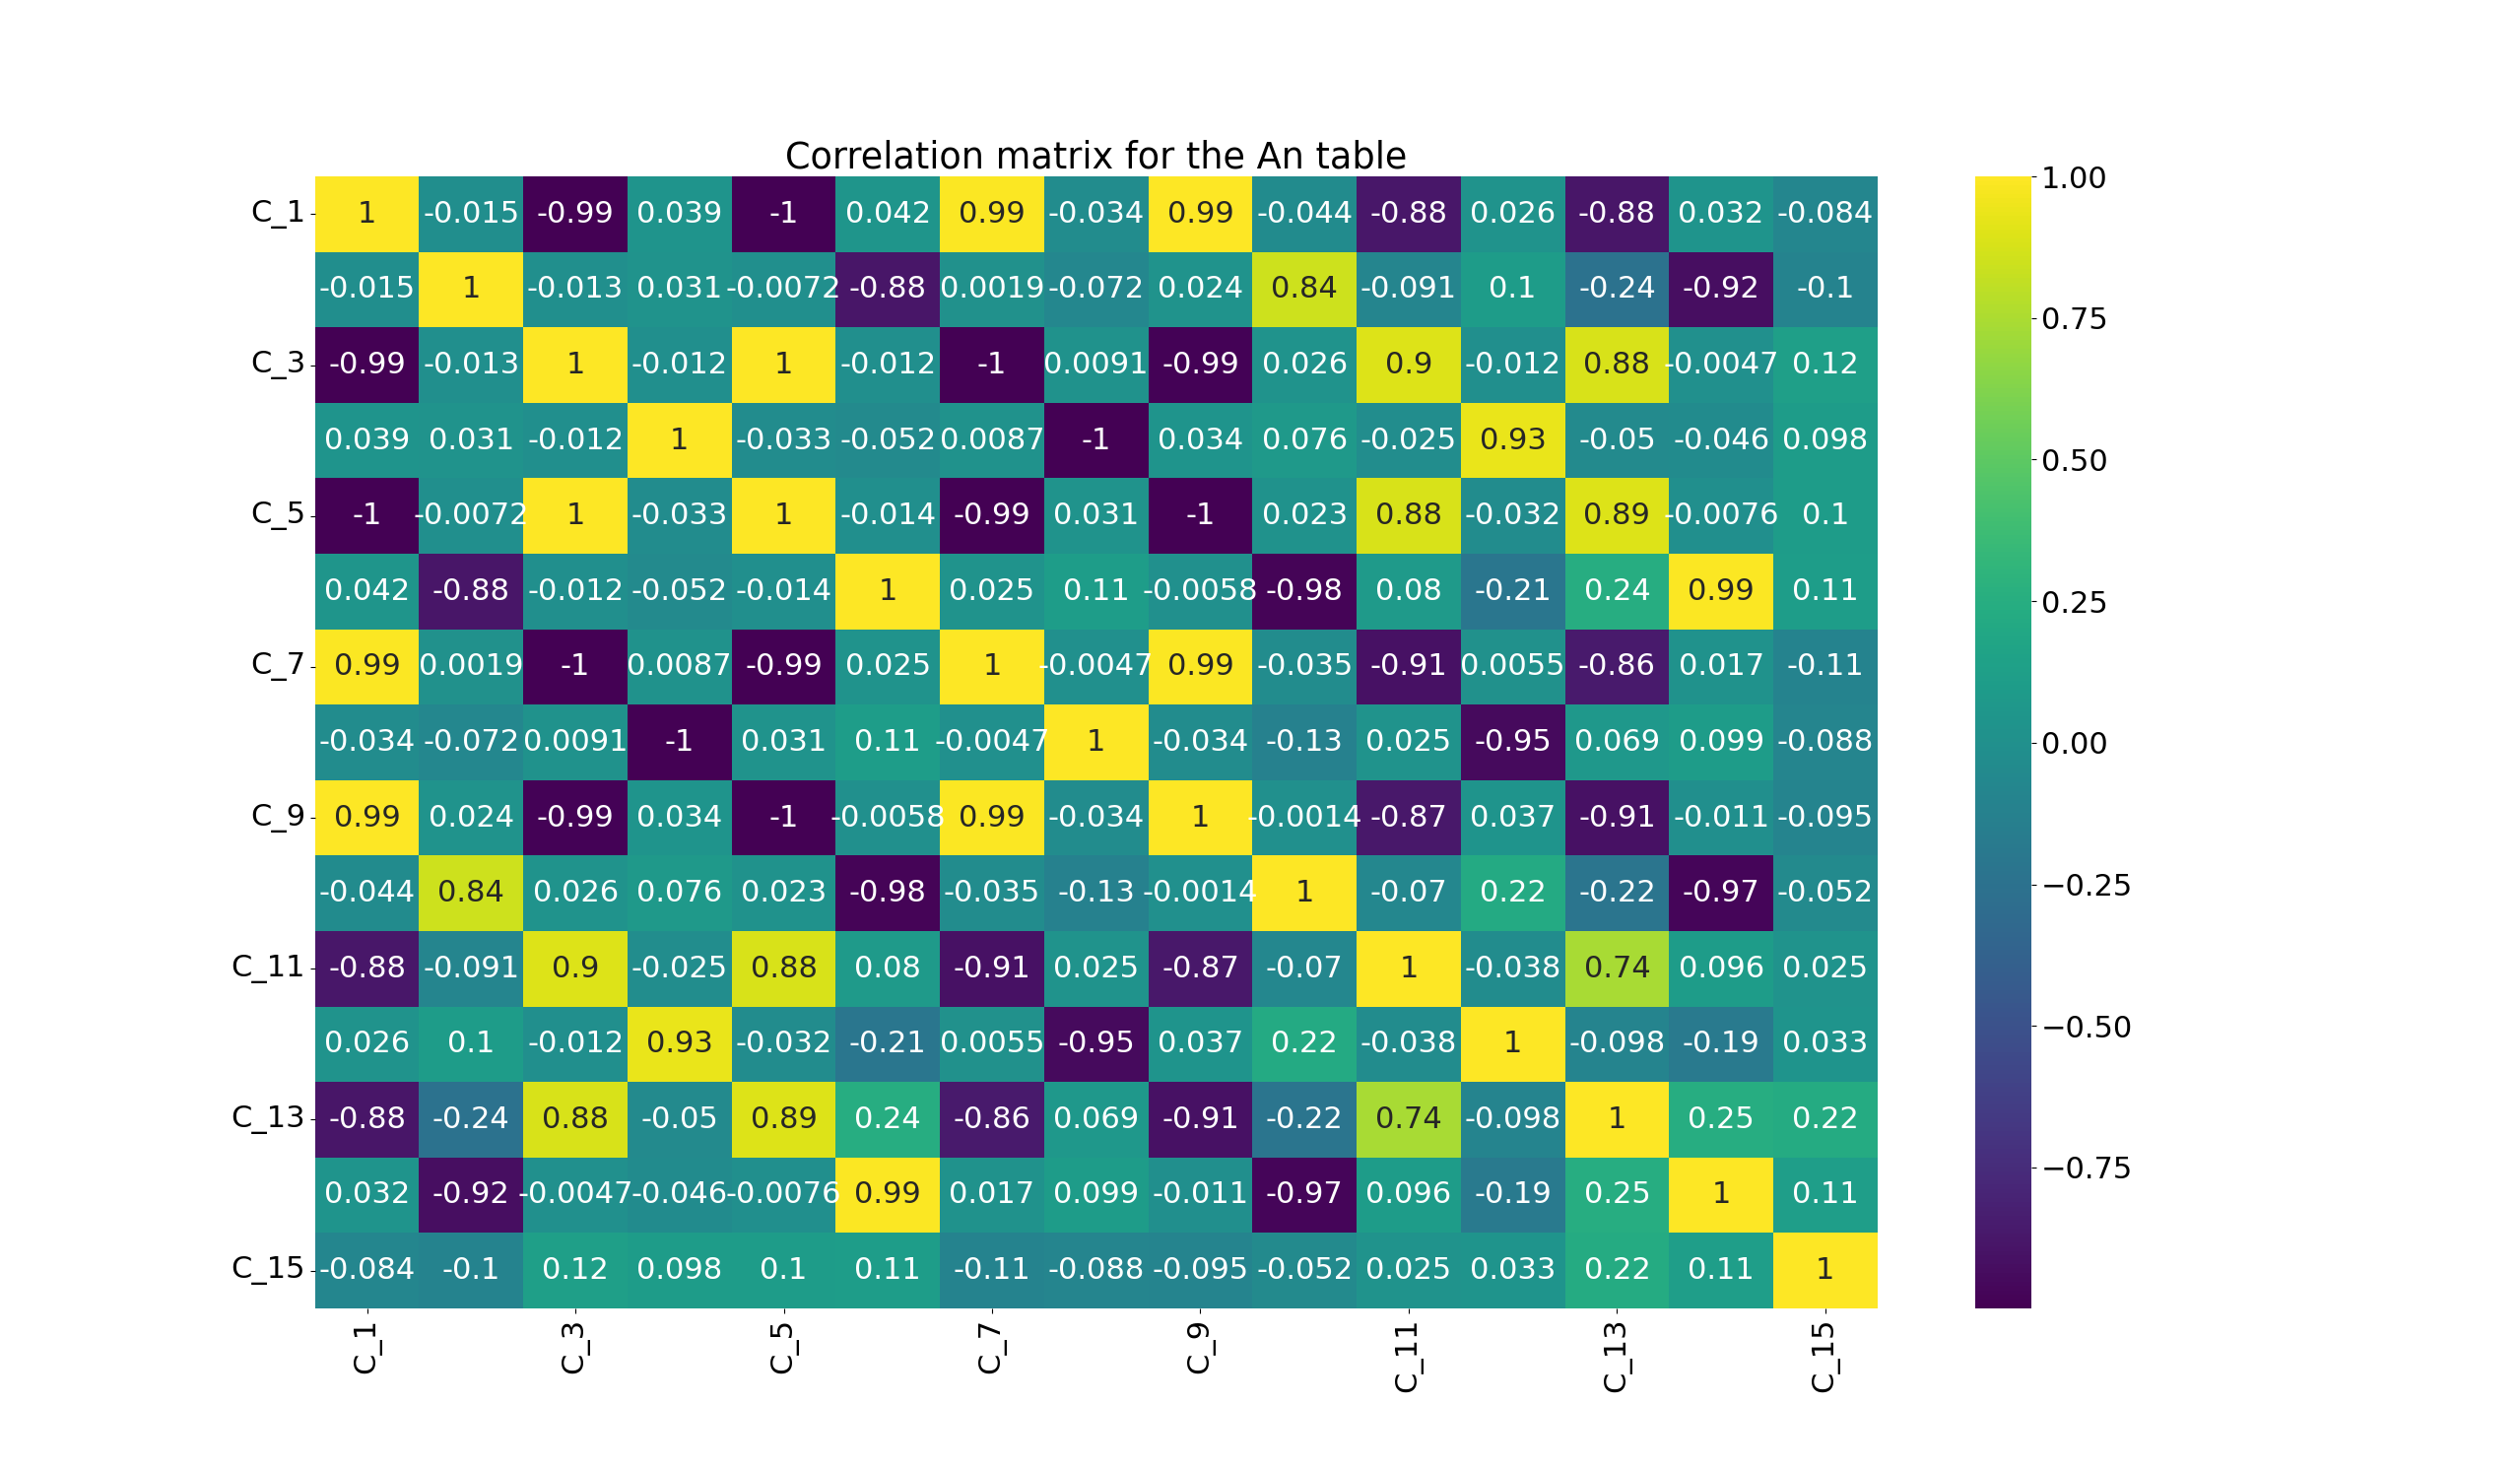
\includegraphics[width=\linewidth]{img/An_corr_matrix.png}
	\caption{The cross-correlation of the \an\ harmonics} \label{fig:an-corr}
\end{figure}

By looking at \Cref{fig:an-corr} we can gather the following information:
\begin{itemize}
	\item Its strong geometry implies that doing feature extraction is going to be complex, due to the necessity of finding a mix of harmonics that has a high correlation with the label, while having a low correlation among themselves.
	\item All the odd harmonics are strongly correlated with each other (with the sole exception
	      of harmonic $15$),
	\item Harmonic number $2$ is strongly correlated with its odd multiples,
	\item Harmonic number $4$ is strongly correlated with all its multiples,
	\item Harmonic number $15$ is the only one that is not correlated to any of the other
	      harmonics.
\end{itemize}

\Cref{fig:an-lcorr} aims to show how informative the various harmonics with regard to the single
label ('quench' or 'non-quench').

\begin{figure}
	\centering
	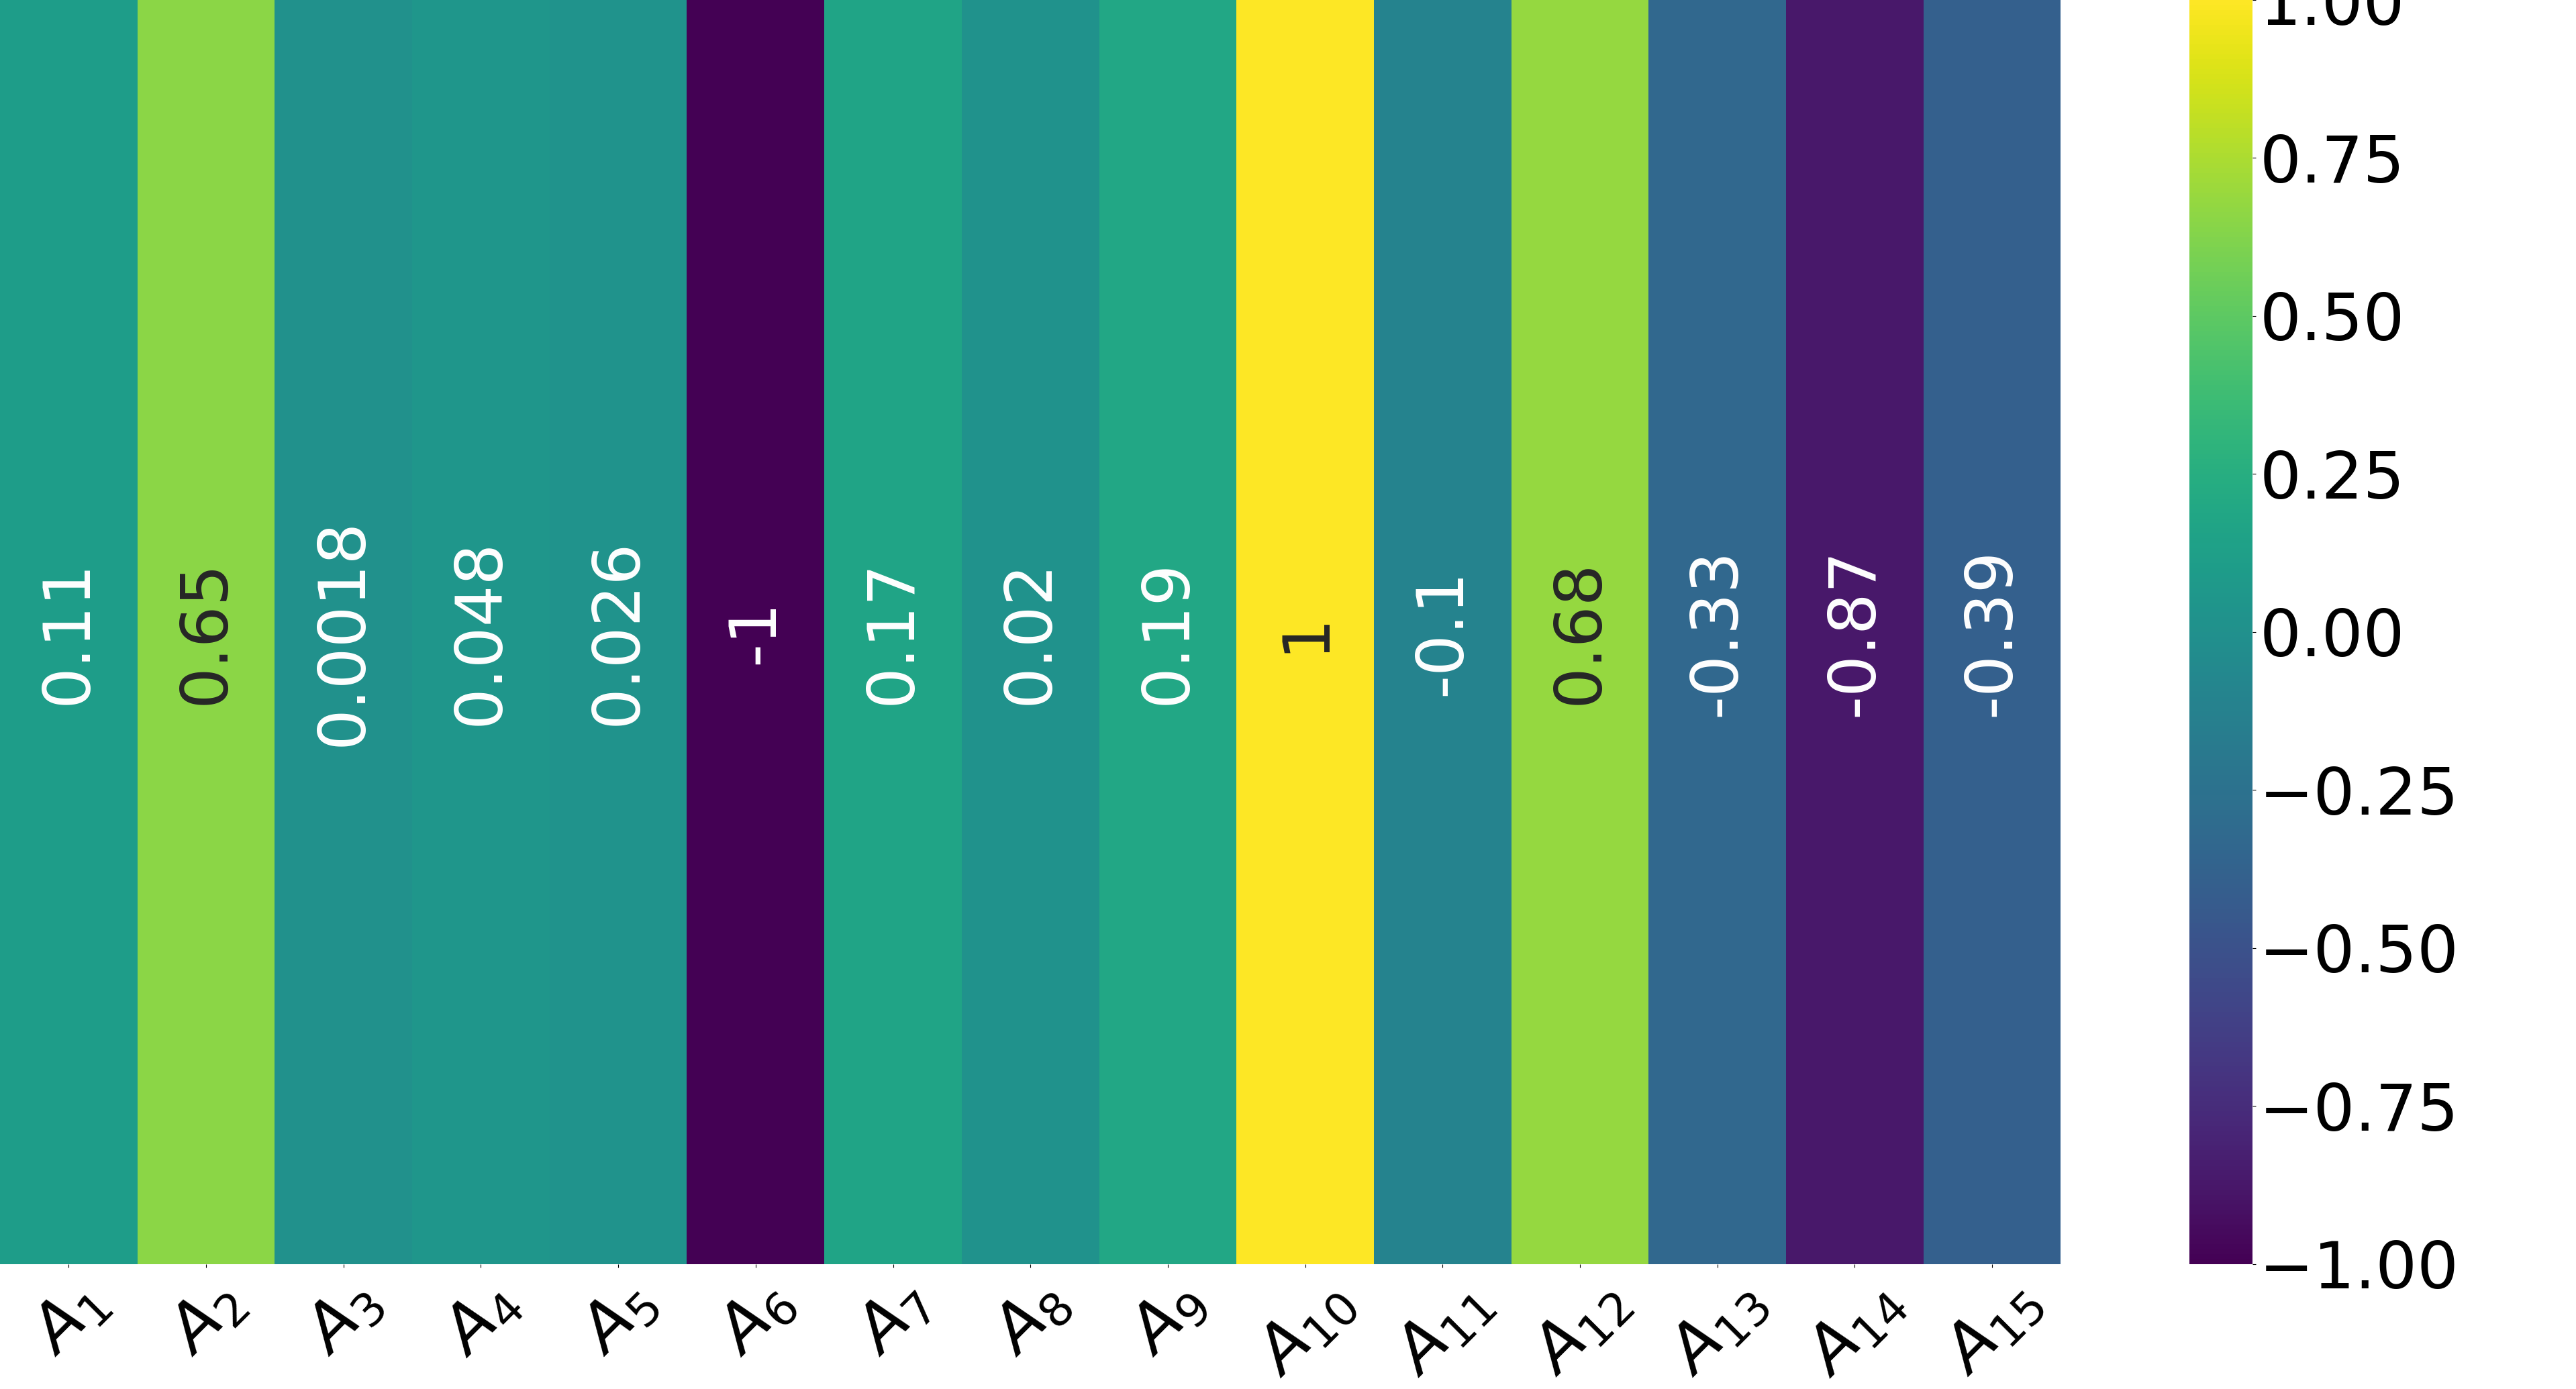
\includegraphics[width=\linewidth]{img/An_label_corr.png}
	\caption{Label correlation for the \an\ table} \label{fig:an-lcorr}
\end{figure}

Once again, considering \Cref{fig:an-lcorr}, we picked the harmonics with the highest label
correlation, which are identified by a higher color intensity; as we can see the label is explained
very well by harmonics number: $2, 6, 10, 11, 12, 13, 14, 15$.
These conclusions are doubly interesting, since:
\begin{enumerate}
	\item The $2^{nd}$ harmonic, as well as its odd multiples, can explain the results well, which
	      is what we expect from the theory.
	\item High order harmonics are able to explain the results better than other harmonics,
	      which is not what we would have expect, since in the original analysis the value for the
	      labels was computed using primarily lower order harmonics.
\end{enumerate}

Based on all the information obtained up to this point we can conjecture that some of the best
datasets will probably contain the second harmonic, or one of its high order odd multiples, as well
as harmonic number $15$, and some other high order harmonic (i.e.: harmonics number $11$ or $13$). As we will see
in the following one of the best datasets that we built on this table was based on harmonics $2, 12$.

Lastly, we can visualize the distribution of the samples in bidimensional space, which was achieved
by using a dimensionality reduction technique, namely $\textsc{pca}$ (Principal Component Analysis).
\begin{figure}[h!]
	\centering
	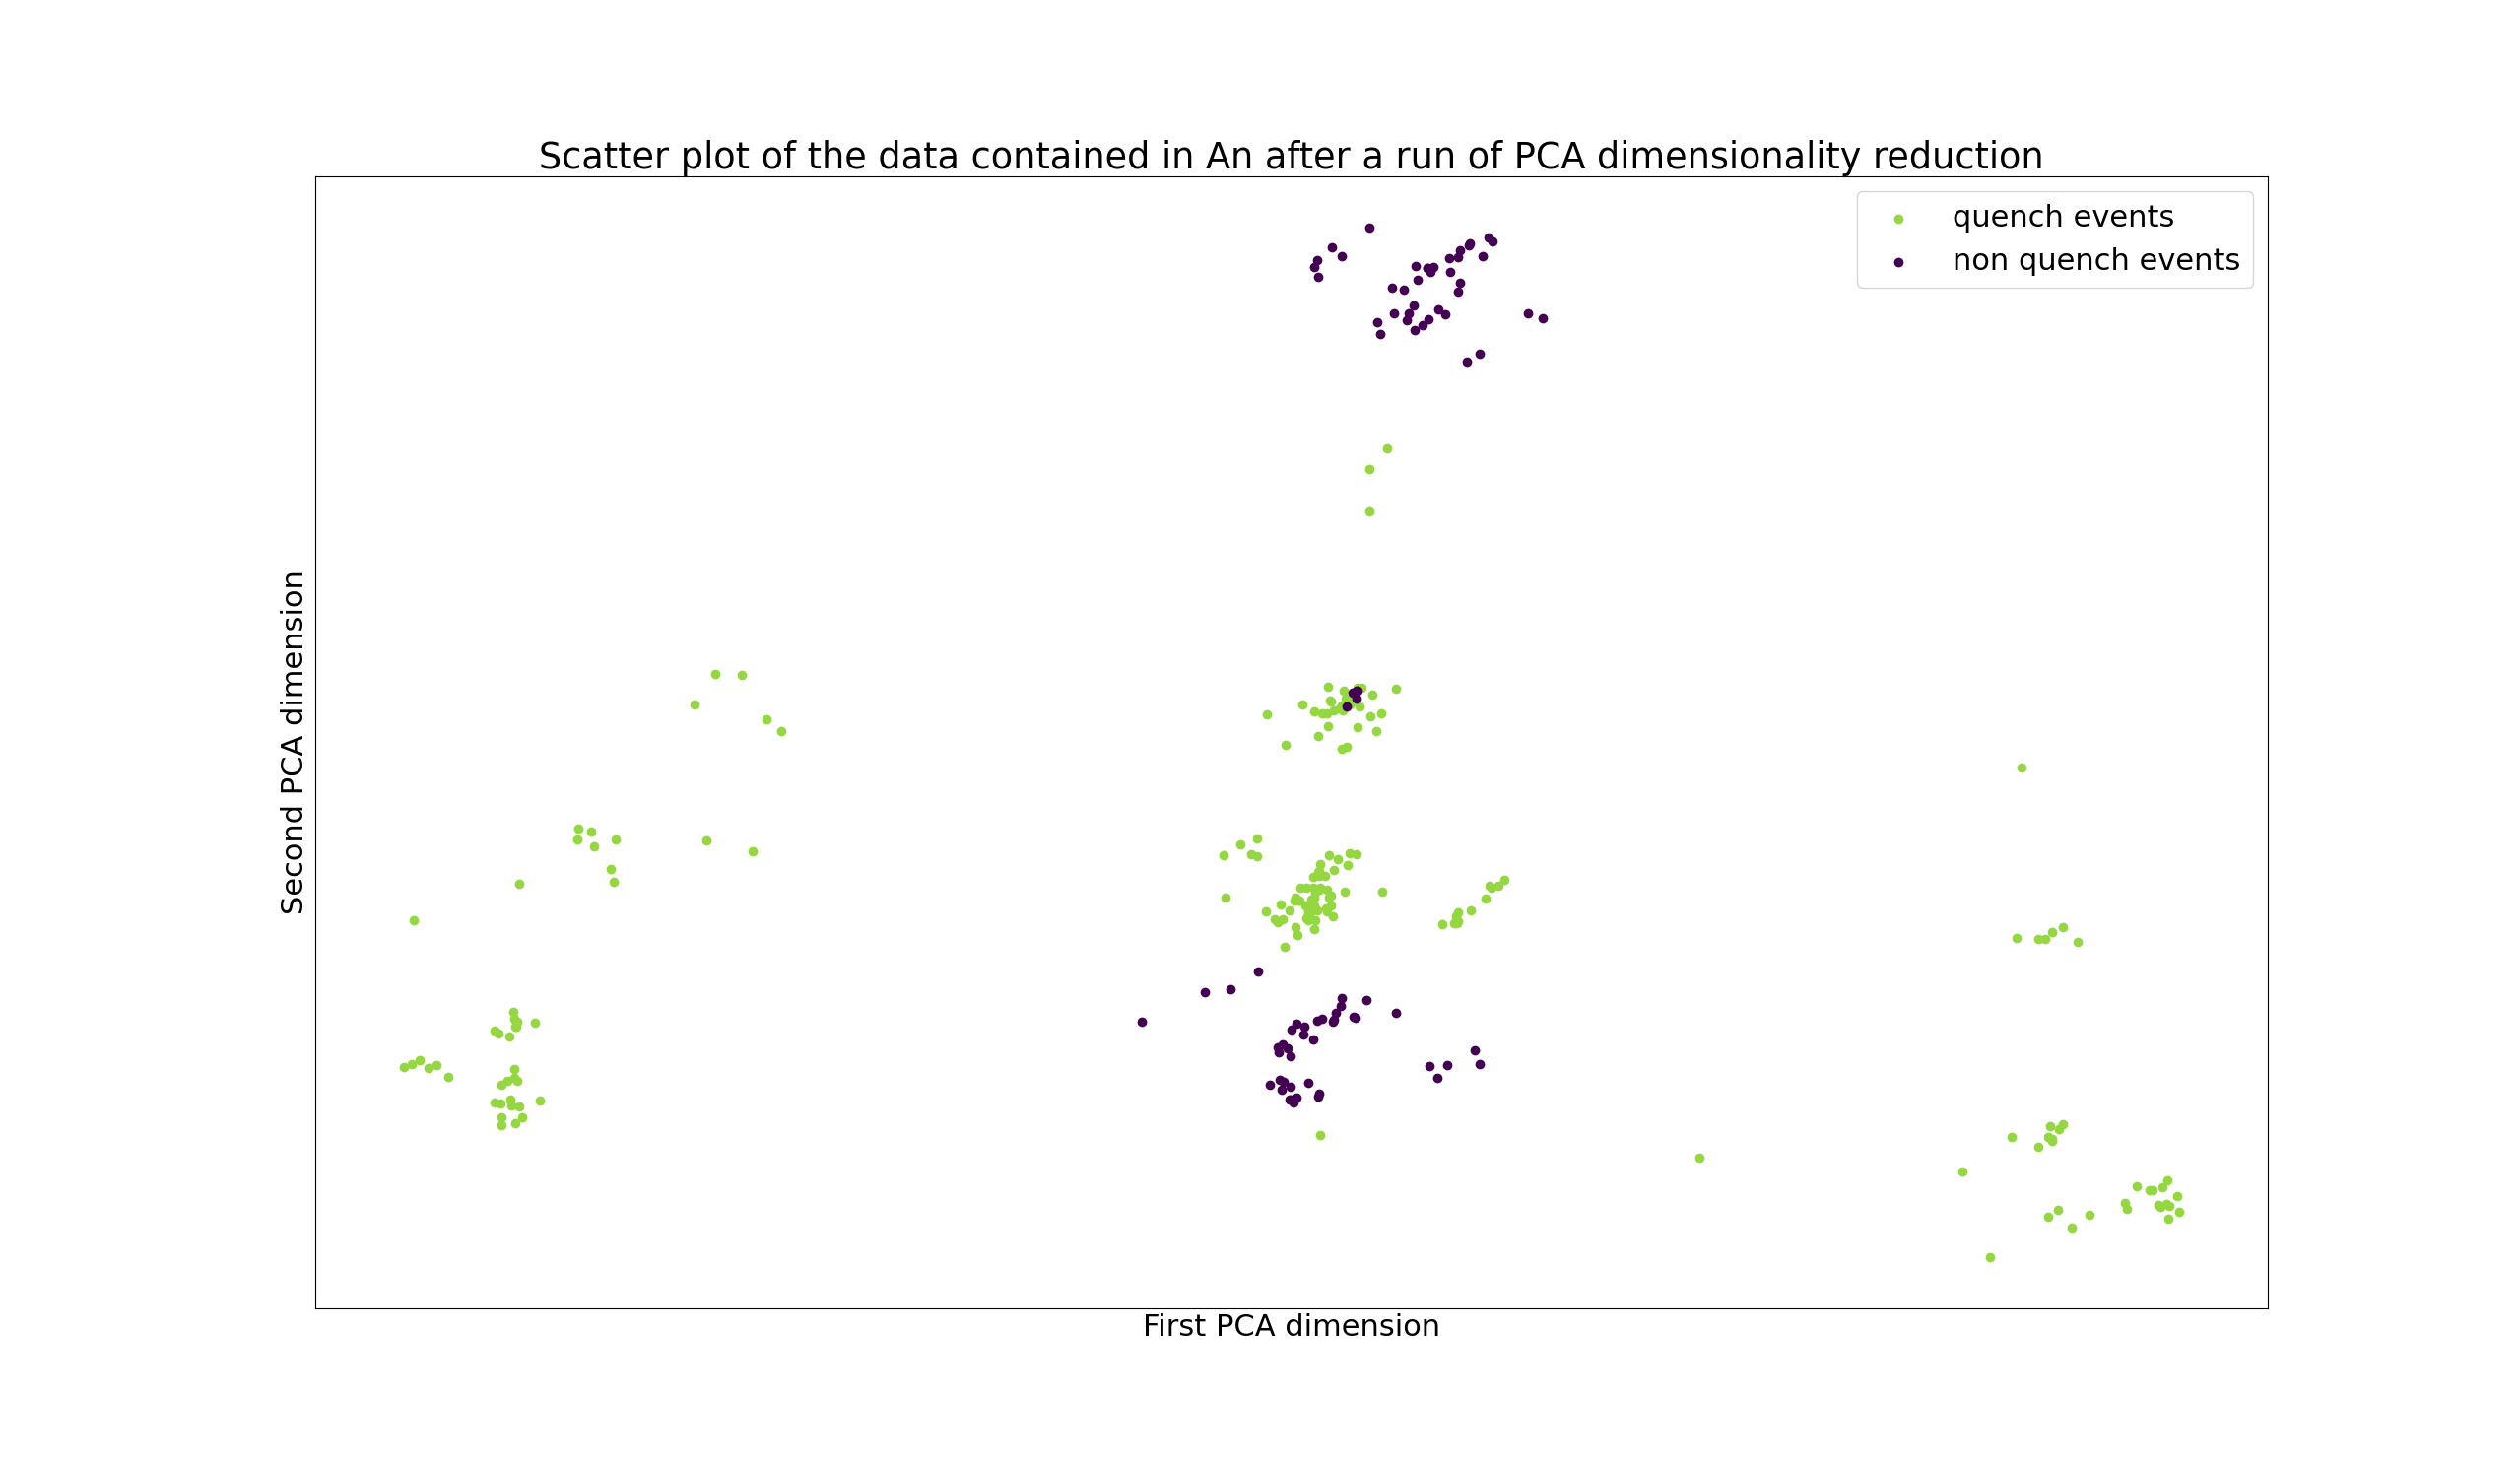
\includegraphics[width=\linewidth]{img/An_distribution.png}
	\caption{Data distribution for the \an\ table after applying $\textsc{pca}$ dimensionality
		reduction} \label{fig:an-dist}
\end{figure}

It can be seen in \Cref{fig:an-dist} that the samples, after dimensionality reduction, are distributed very nicely in a series
of zones, each zone has a very high degree of purity; this lead us to suppose that it might be the
reason why models built on \an\ and \cnmod\ perform better than the alternatives.

\subsubsection{\bn\ table}
We can use a similar procedure on the \bn\ table, which in most tests proved to be the
least-performing table. This is probably due to the poor distribution of the data, as we can see in
\Cref{fig:bn-dist}, it's really hard to find a way to separate the central portion of the samples.
\begin{figure}[h!]
	\centering
	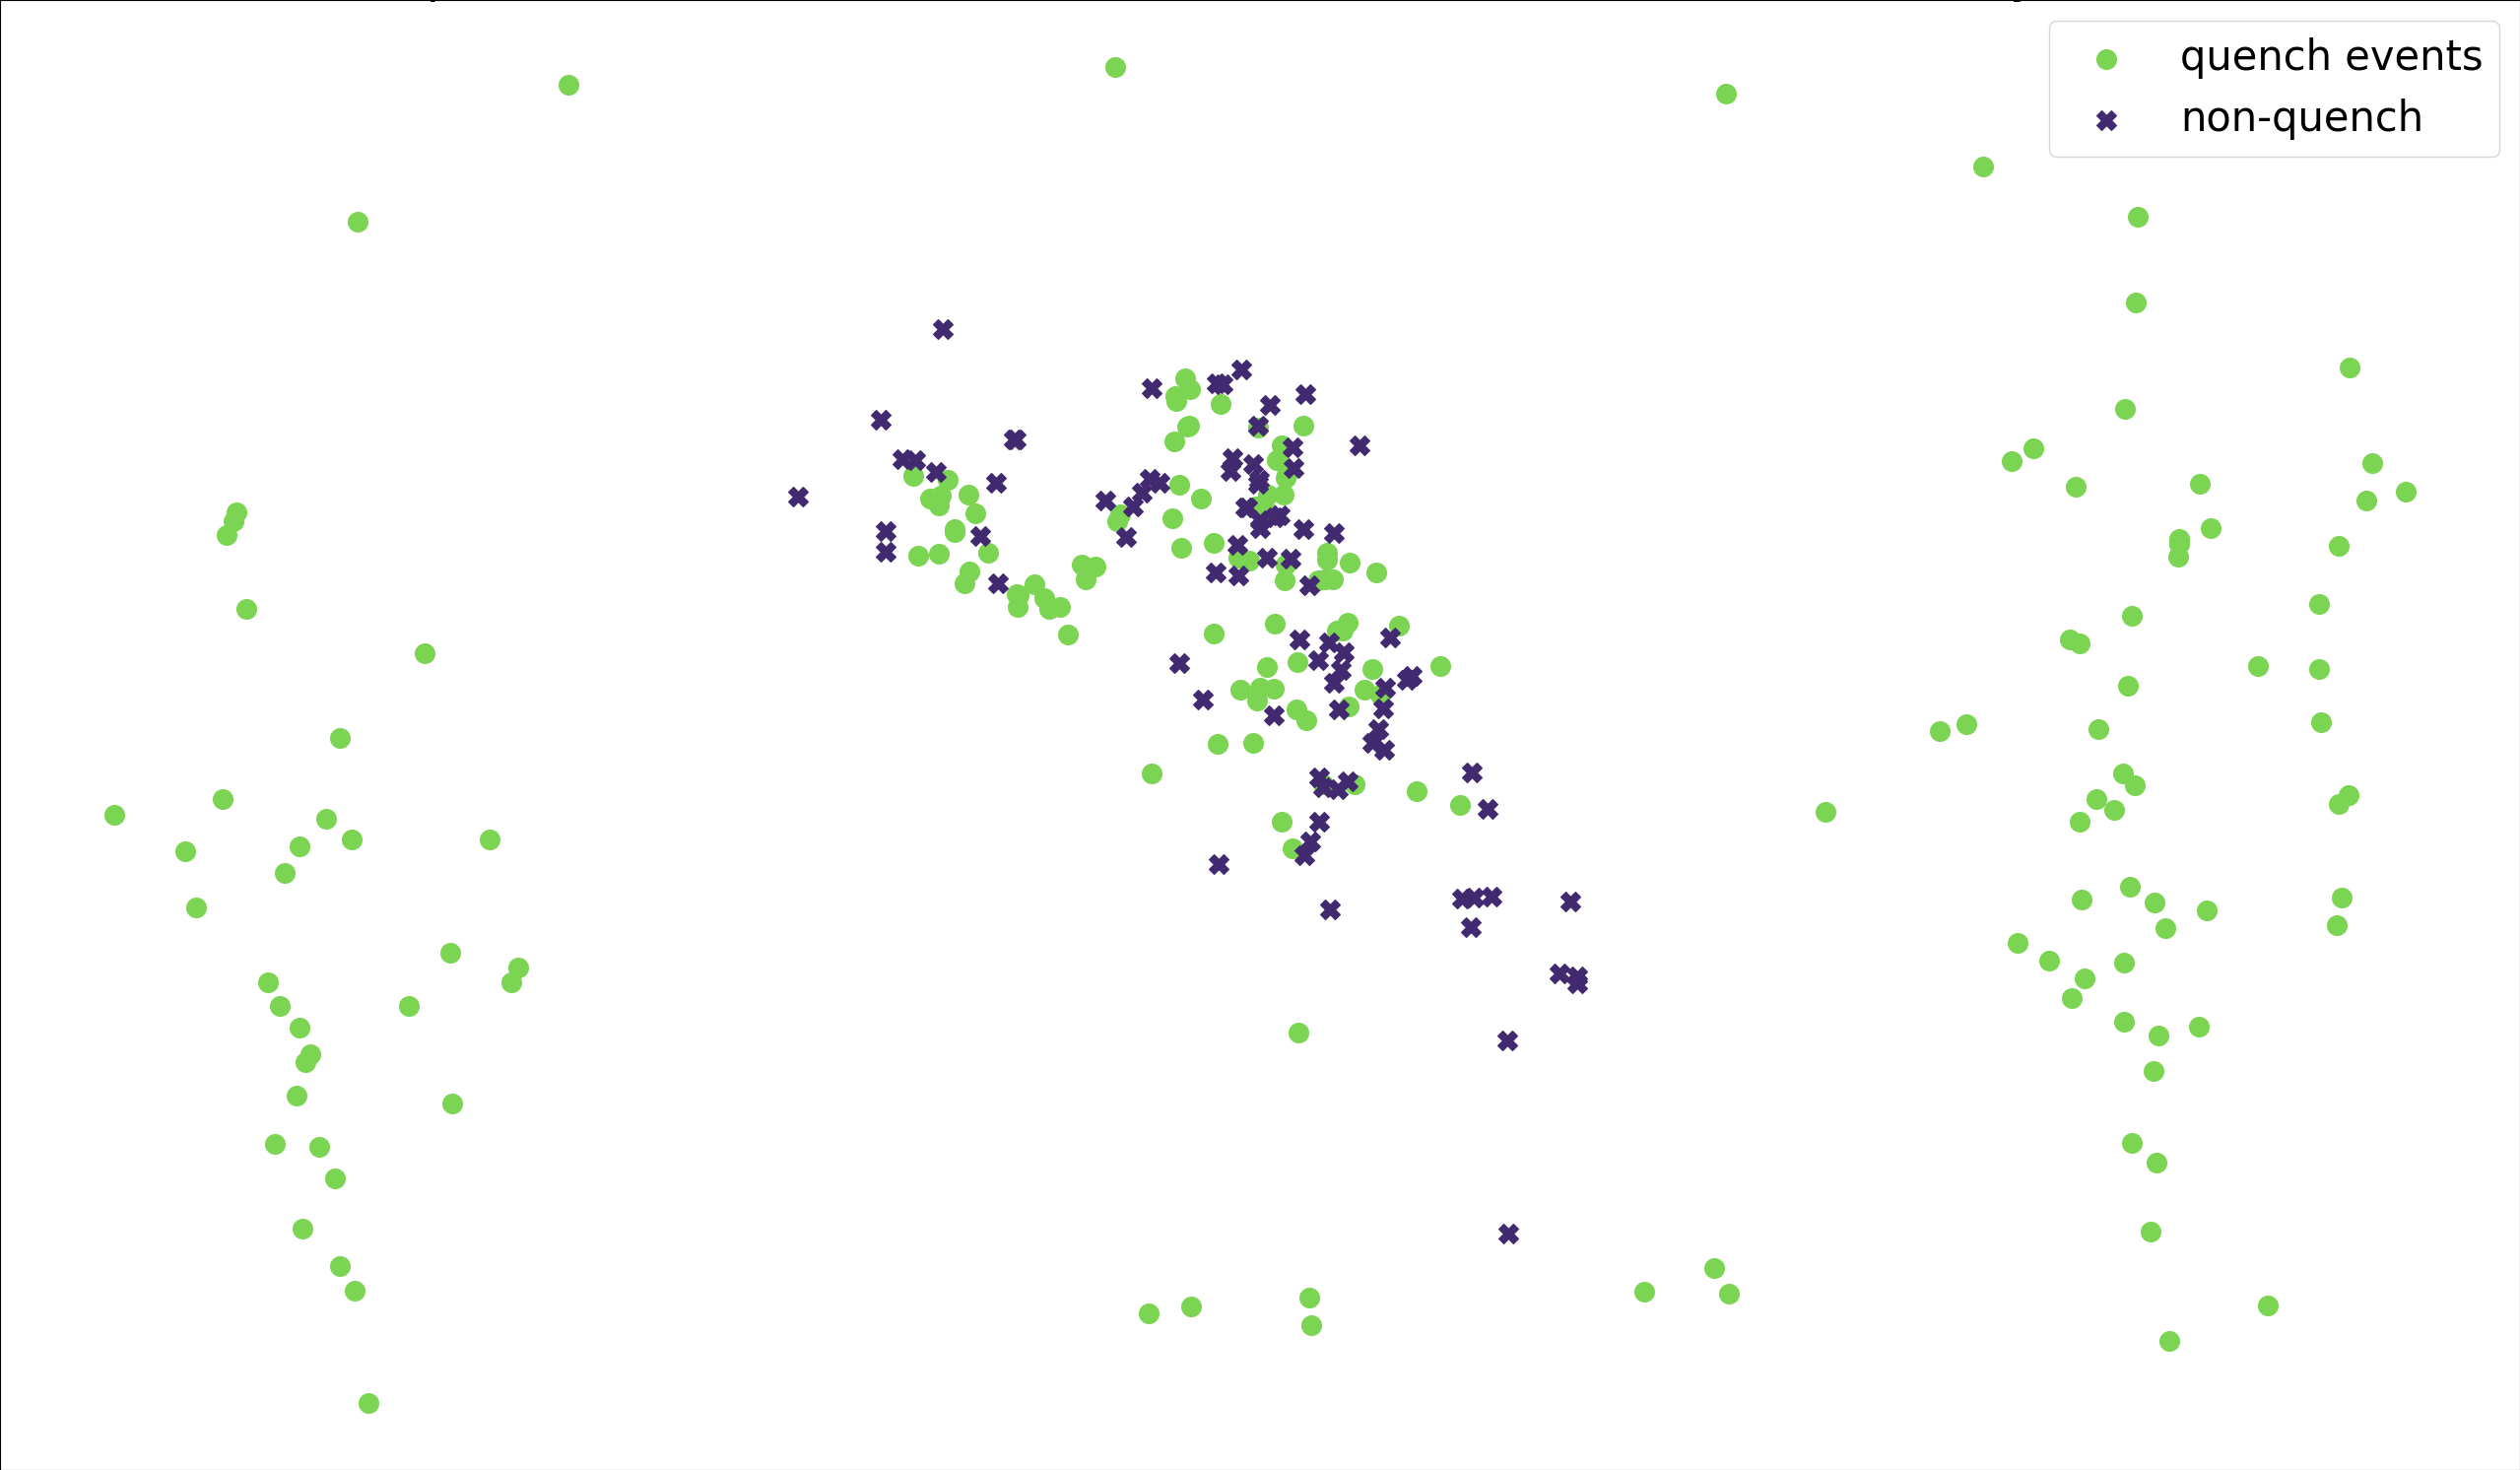
\includegraphics[width=\linewidth]{img/Bn_distribution.png}
	\caption{Data distribution for the \bn\ table after applying $\textsc{pca}$ dimensionality
		reduction} \label{fig:bn-dist}
\end{figure}

As we did for \an\ we checked the cross-correlation of the \bn\ table, and the results were actually very
similar.
\begin{figure}[h!]
	\centering
	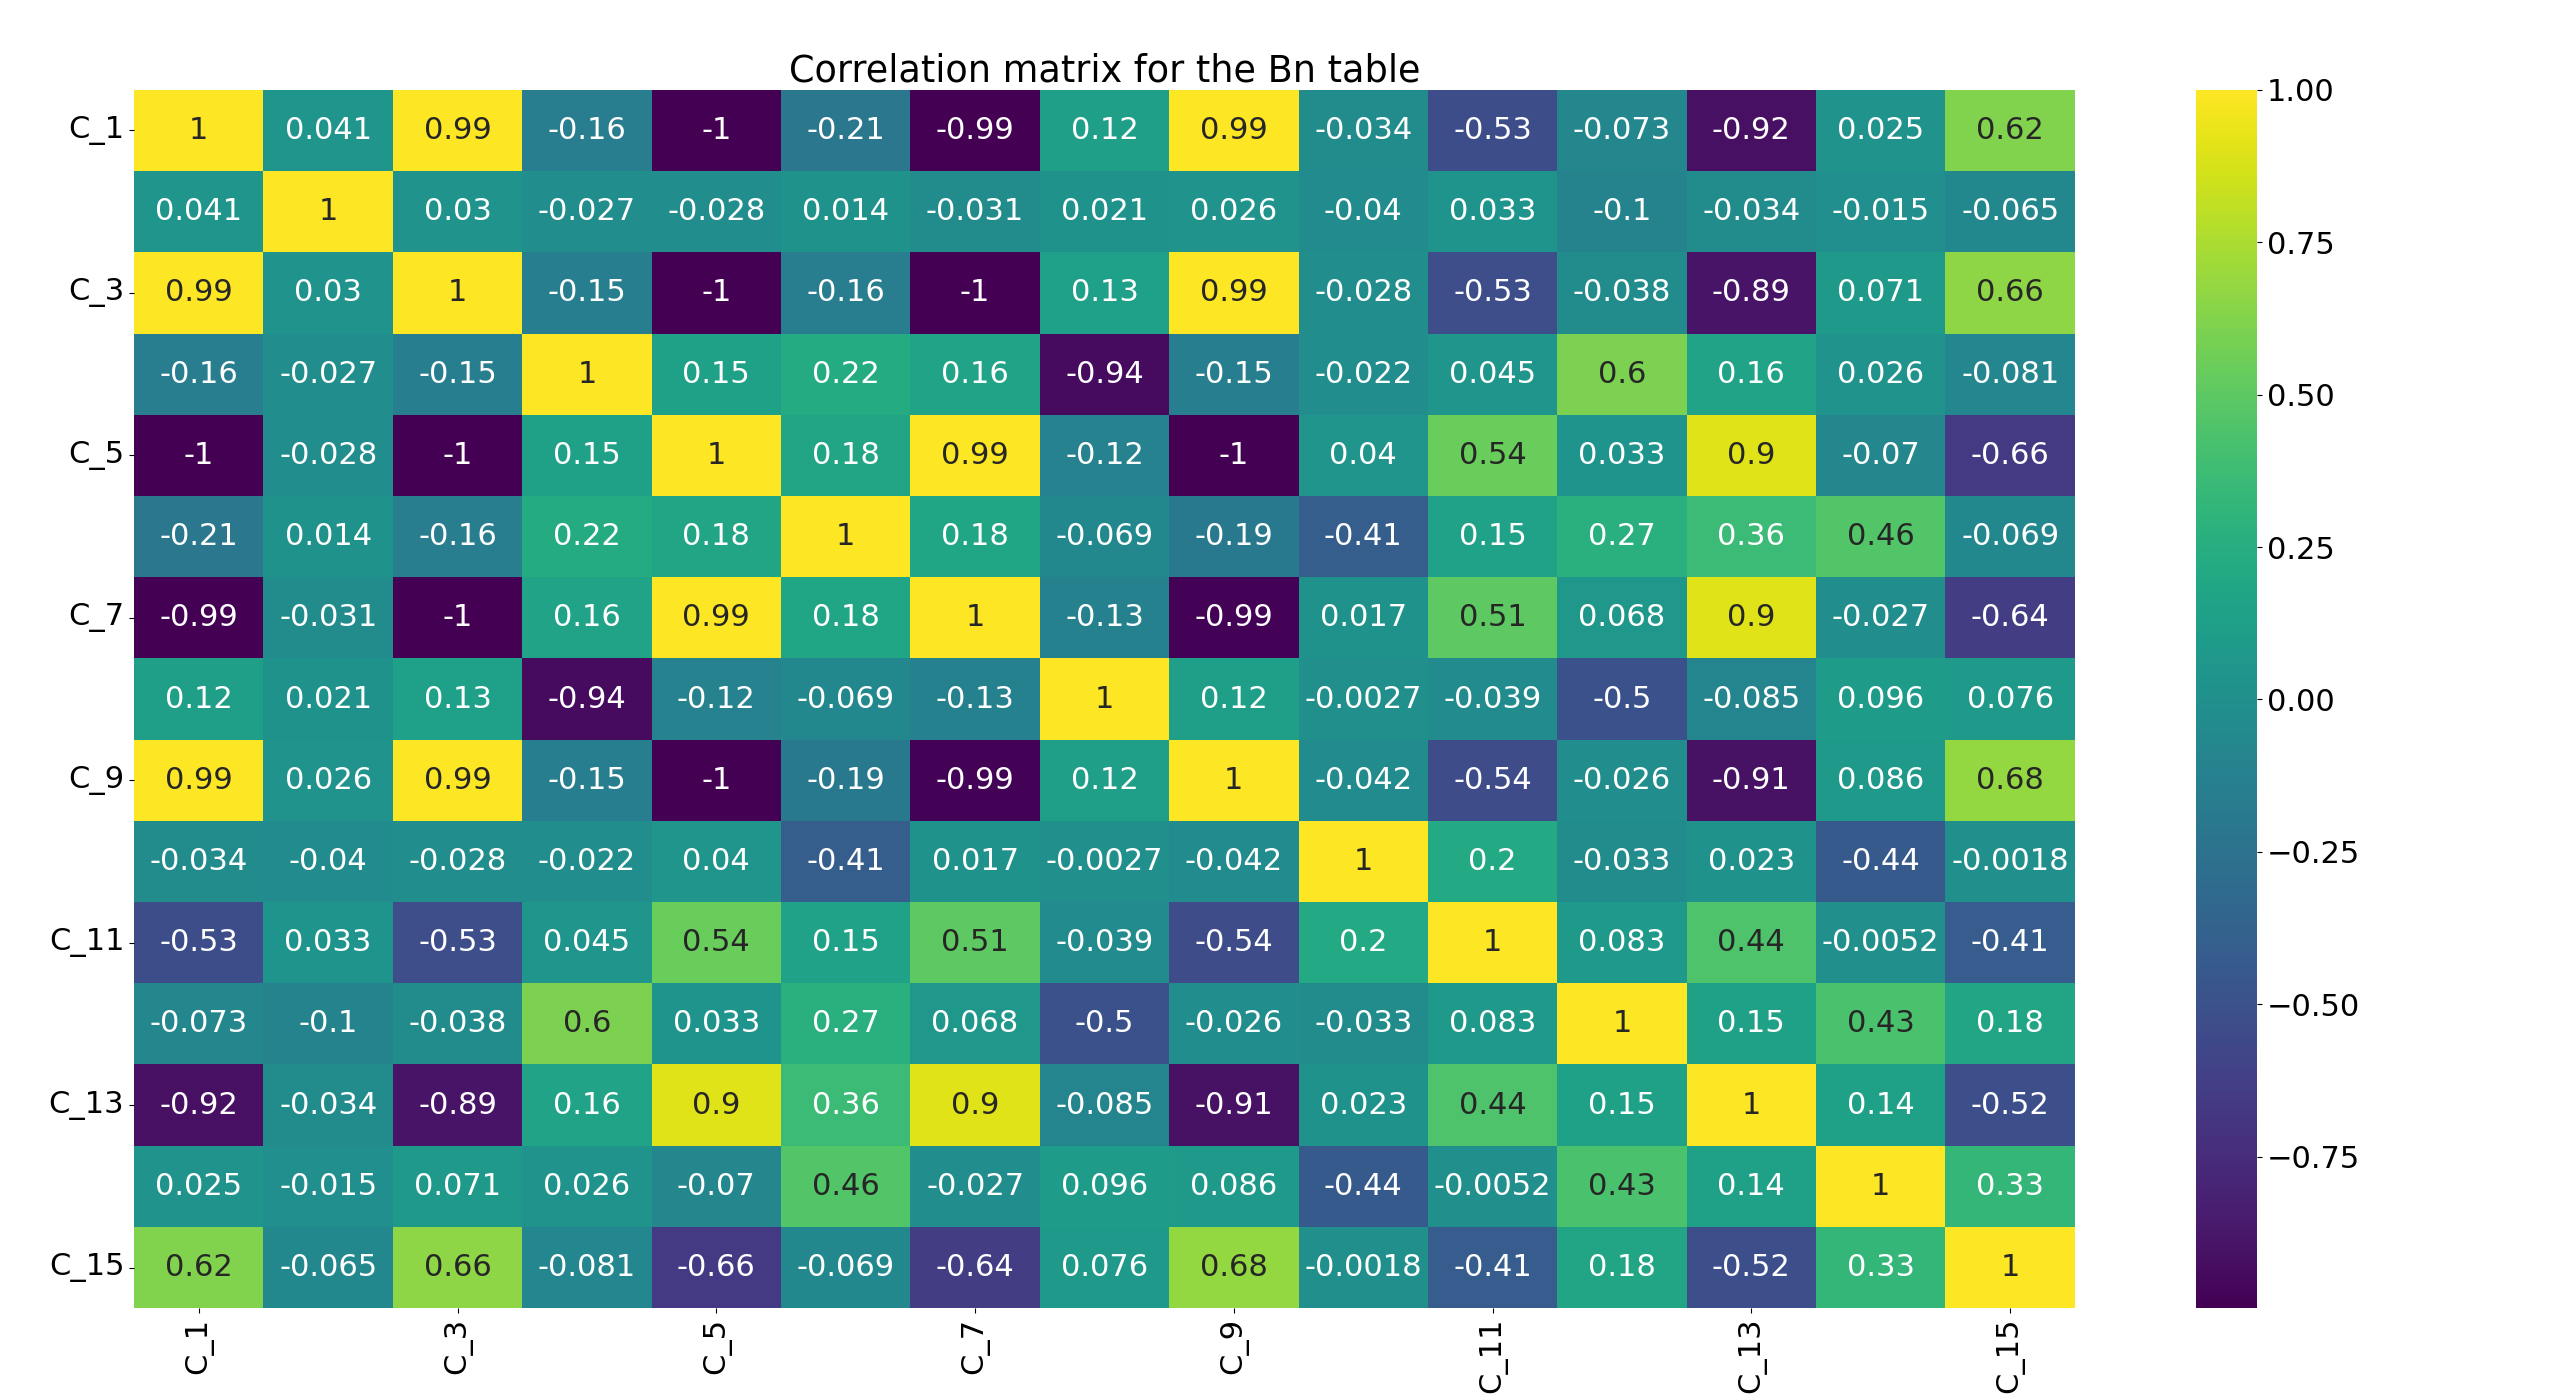
\includegraphics[width=\linewidth]{img/Bn_corr_matrix.png}
	\caption{The cross-correlation of the \bn\ harmonics} \label{fig:bn-corr}
\end{figure}
Possibly the biggest difference between \Cref{fig:an-corr} and \Cref{fig:bn-corr}, apart from the
obvious difference in the correlation values, is that harmonic $2$ is not strongly correlated with
any other harmonic, while harmonic number $15$ grows a discrete correlation with all odd harmonics.

If we check the correlation of the harmonics with the labels in (\Cref{fig:bn-lcorr}), we can see
that, apparently, most harmonics have a good enough correlation with the solution, but despite this, the performance of all
models built on \bn\ suffered.
\begin{figure}
	\centering
	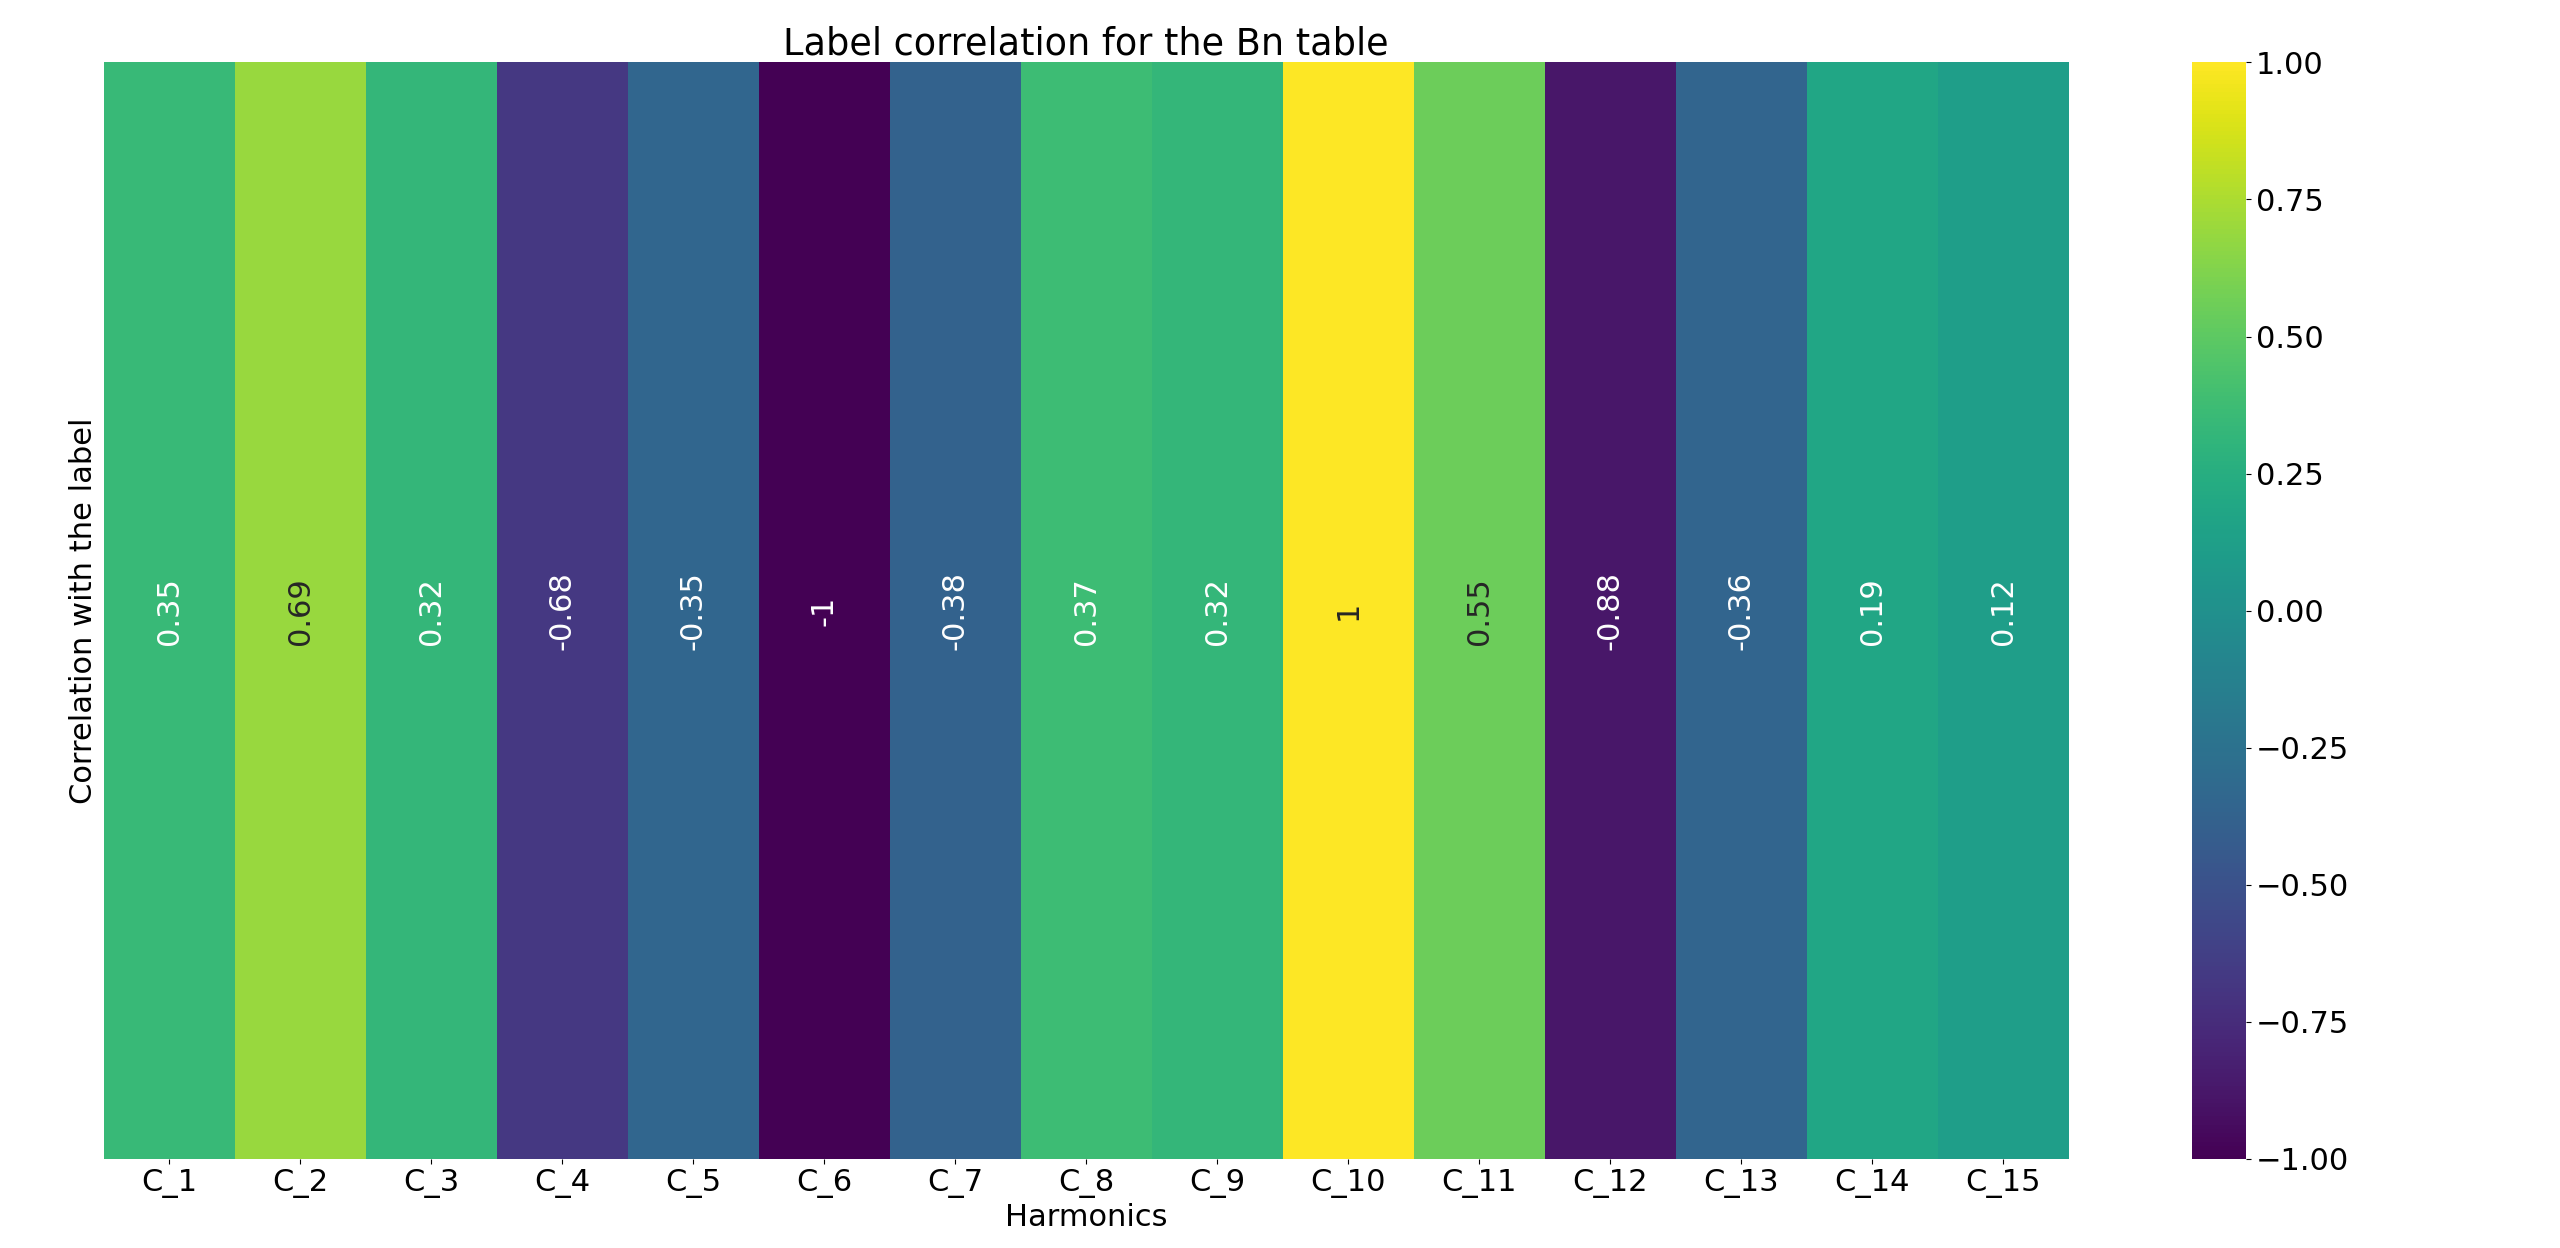
\includegraphics[width=\linewidth]{img/Bn_label_corr.png}
	\caption{Label correlation for the \bn\ table} \label{fig:bn-lcorr}
\end{figure}

\subsubsection{\cnmod\ table}
The \cnmod\ table combines the information present in \an\ and \bn, as we saw in \Cref{sec:dsets},
\cnmod\ was expected to be one of the best tables to solve \qrp, but, as we will see in future
sections, it consistently falls short of the \an\ table, and that is probably due to the
introduction of the information carried by \bn.
\begin{figure}[h!]
	\centering
	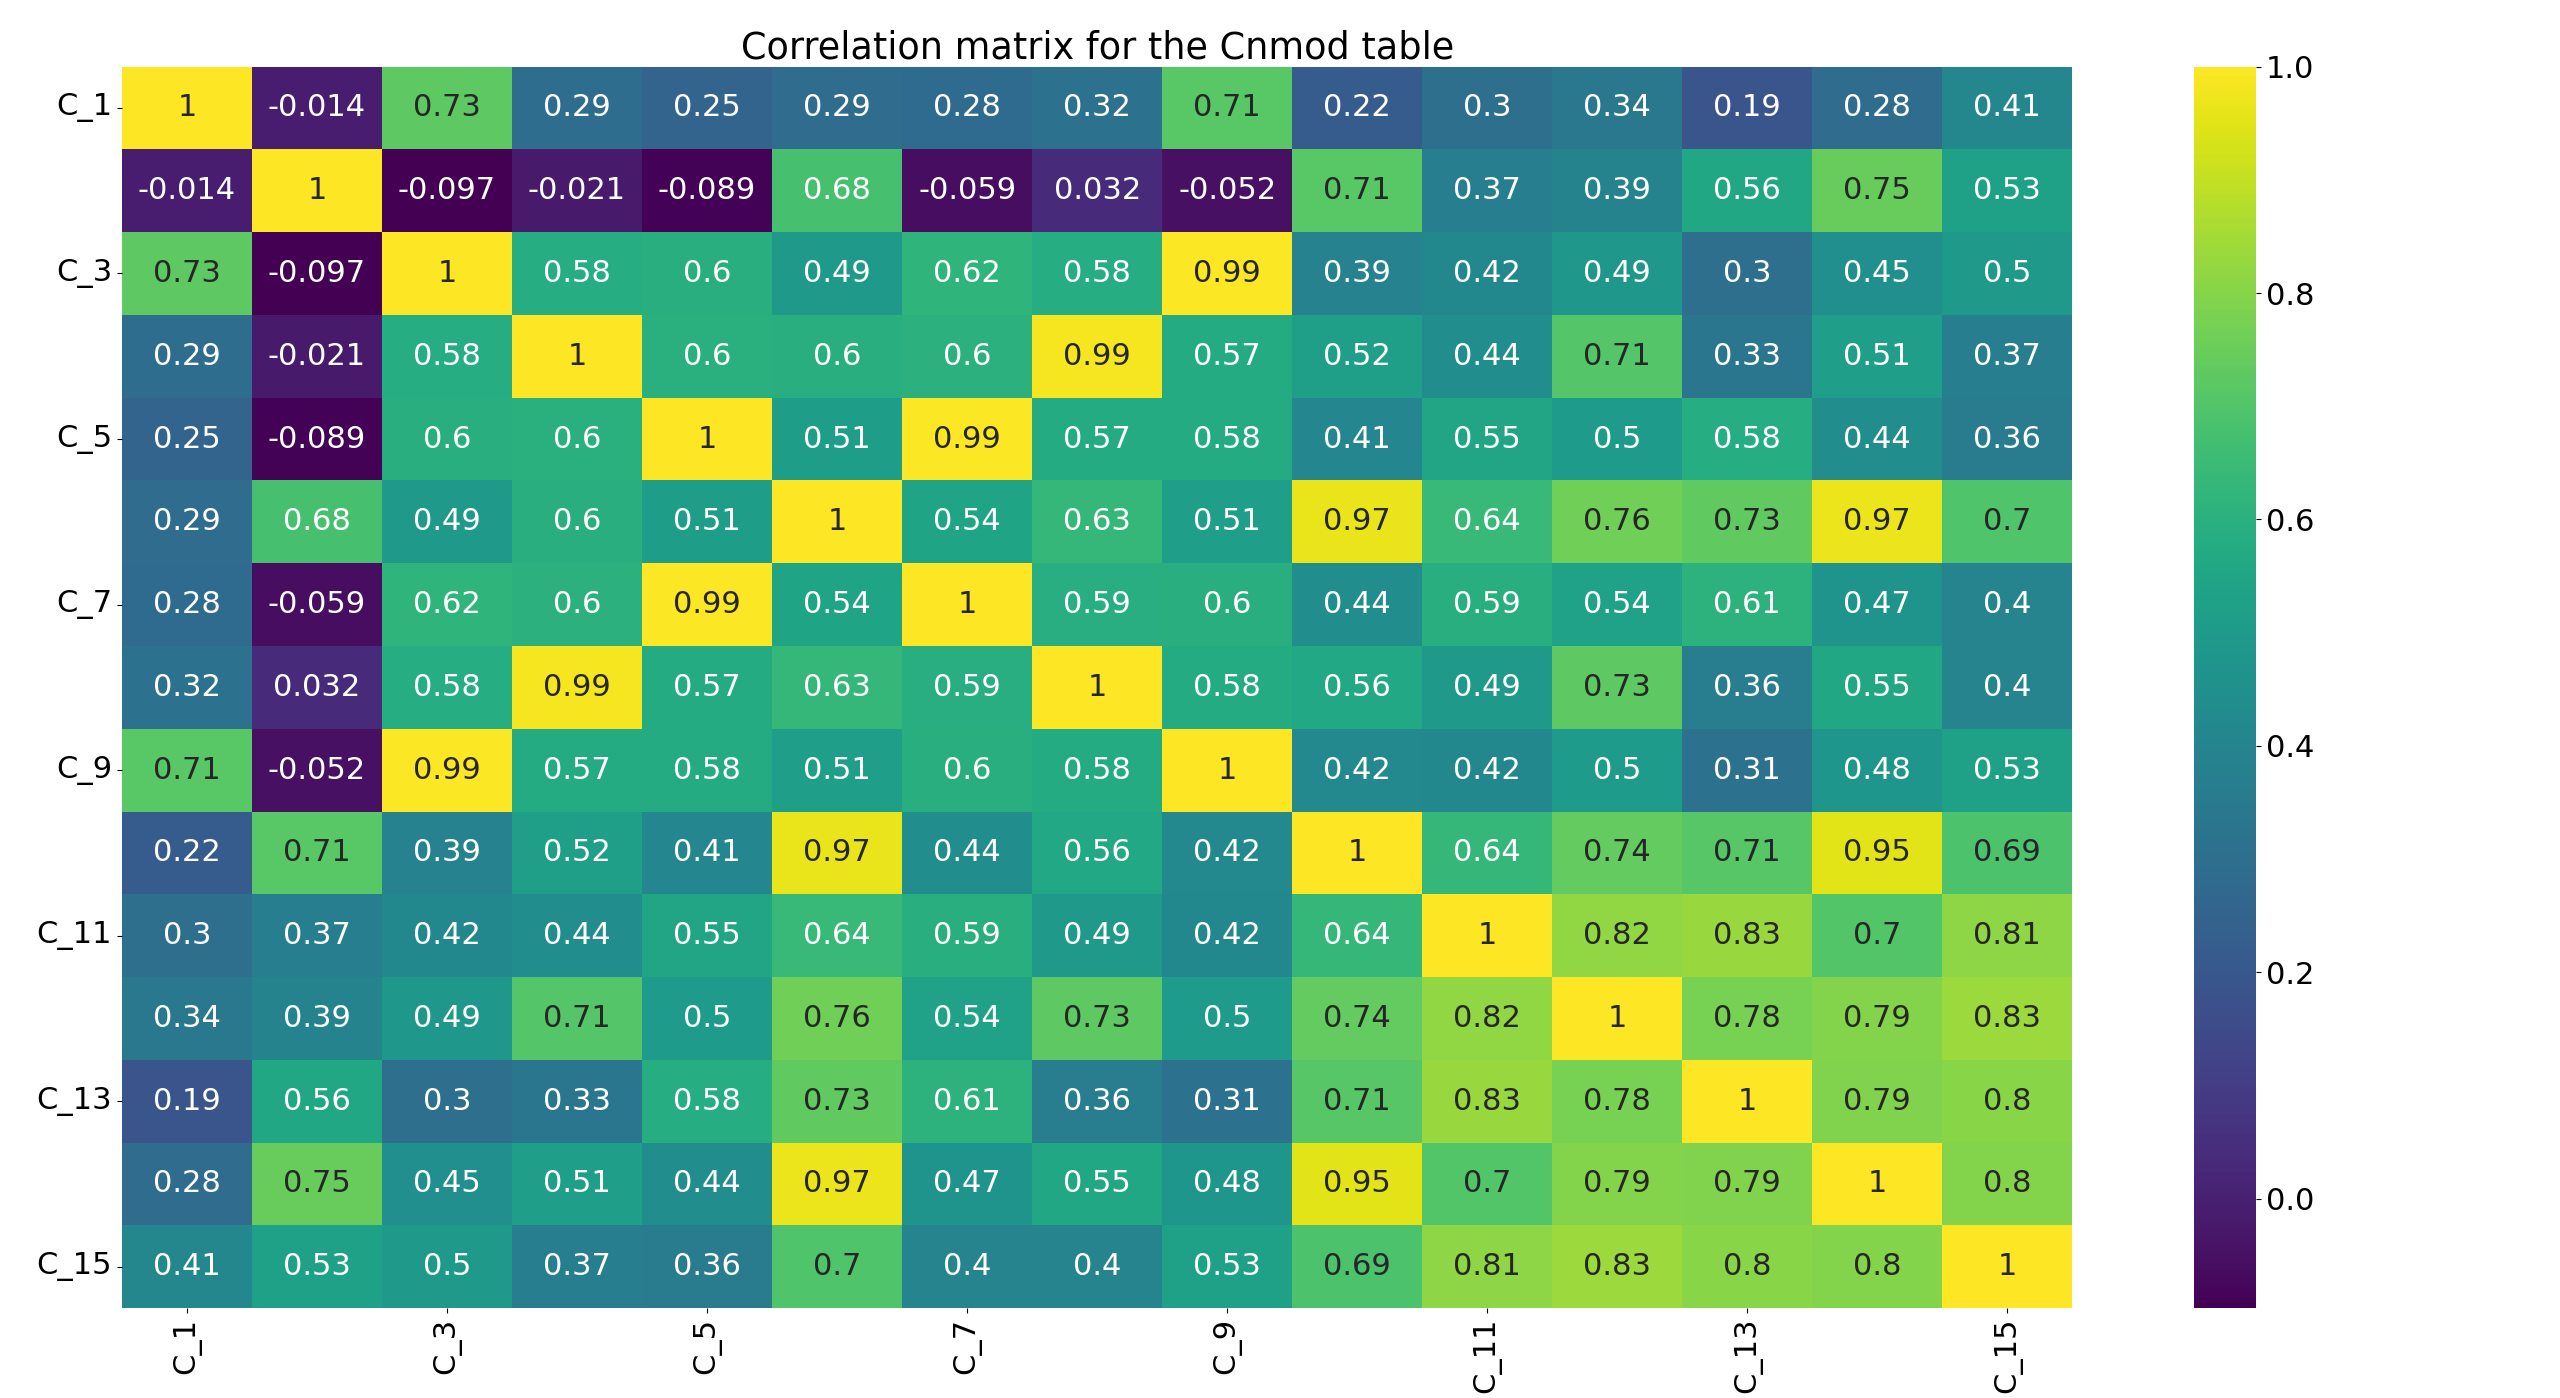
\includegraphics[width=\linewidth]{img/Cnmod_corr_matrix.png}
	\caption{The cross-correlation of the \cnmod\ harmonics} \label{fig:cnmod-corr}
\end{figure}

As we can see in \Cref{fig:cnmod-corr} the correlation matrix for \cnmod\ is very complicated:
\begin{itemize}
	\item Harmonic number $2$ is strongly correlated with any other harmonic until number $9$,
	\item Harmonics between $10$ and $15$ are strongly correlated among themselves,
	\item Harmonic number $4$ is strongly correlated with its multiples.
\end{itemize}

If we check the correlation between the harmonics and the labels \Cref{fig:cnmod-lcorr} we can see
that the first harmonics explain really well the expected results.
\begin{figure}[h!]
	\centering
	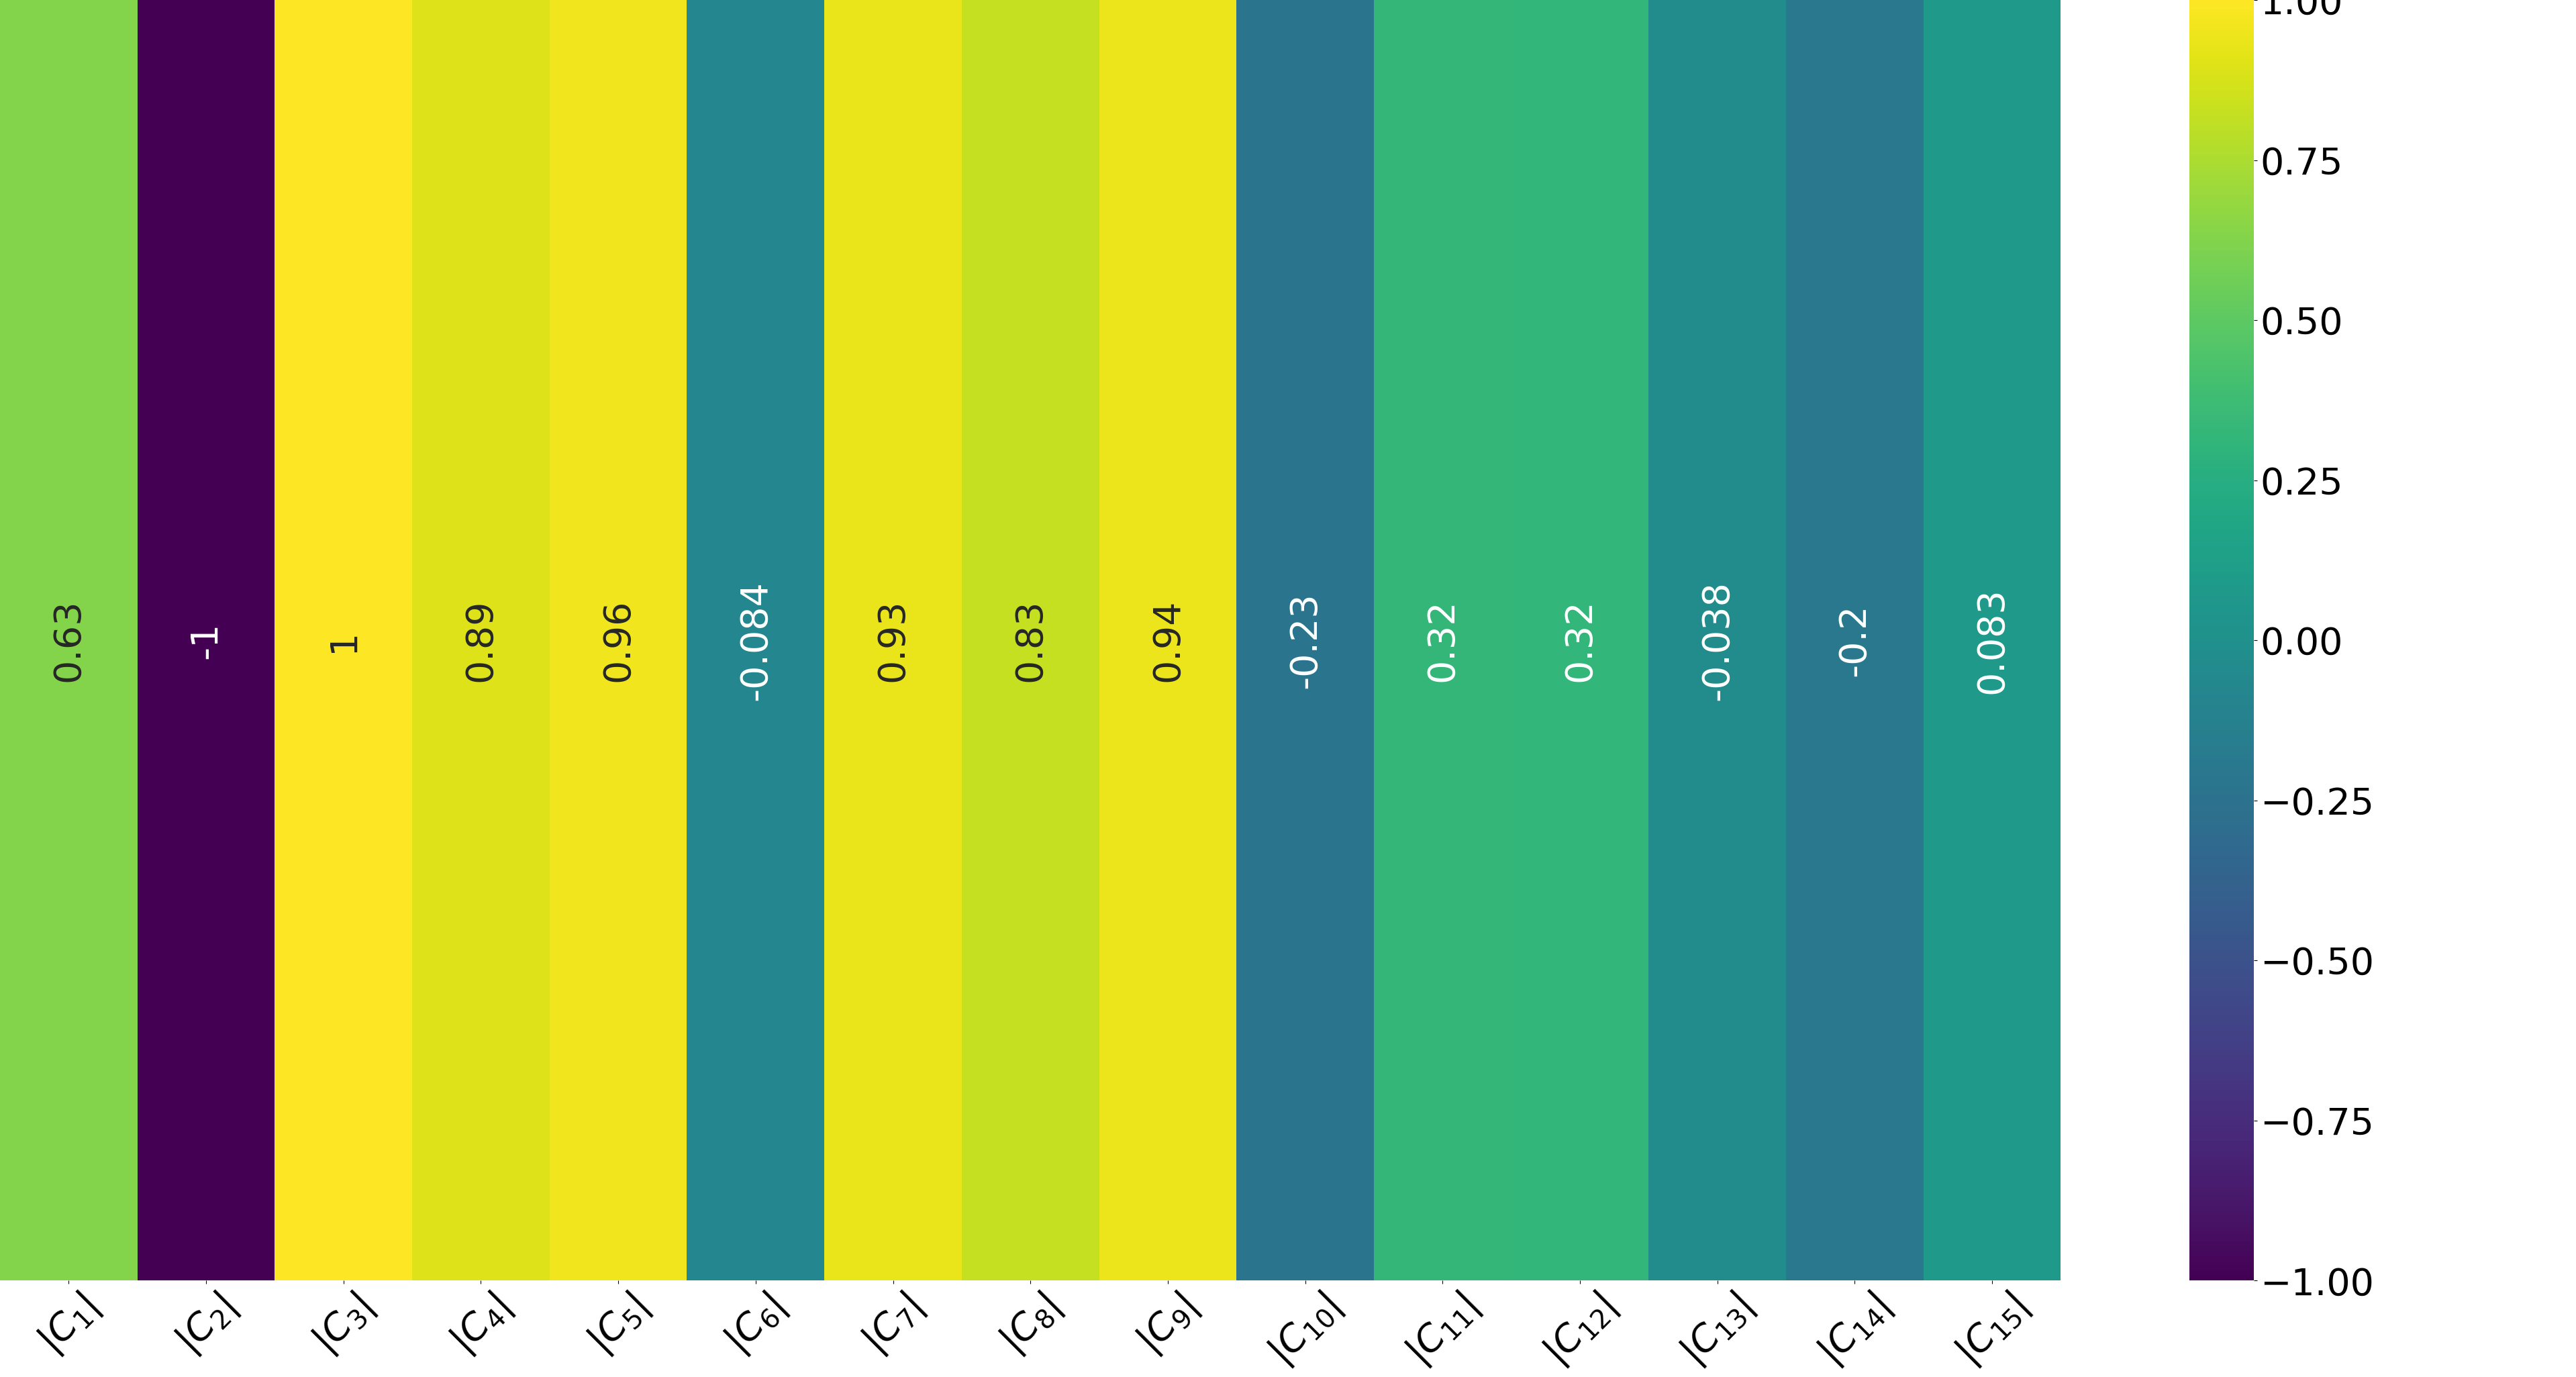
\includegraphics[width=\linewidth]{img/Cnmod_label_corr.png}
	\caption{Label correlation for the \cnmod table} \label{fig:cnmod-lcorr}
\end{figure}

Looking at both \Cref{fig:cnmod-corr} and \Cref{fig:cnmod-lcorr}, we can conclude that two different
approaches could be followed:
\begin{itemize}
	\item If harmonic number $2$ carries enough information it can be used in alongside one or
	      more high-order harmonics,
	\item Another route possible is to use harmonic number $3$ and some other low-order
	      harmonics (potentially even the first one) alongside one low-order harmonic (e.g.,
	      $14$).
\end{itemize}
Analyzing the boxplot suggested that following the first path was not a promising idea since the
variability of the second harmonic is not too high to the

As we will see in a future section the choice that yielded the better performance is to use a
dataset based on harmonic $3$.

Before considering the last table let us stop once again to check the distribution of the
dimensionality reduction for \cnmod.
\begin{figure}[h!]
	\centering
	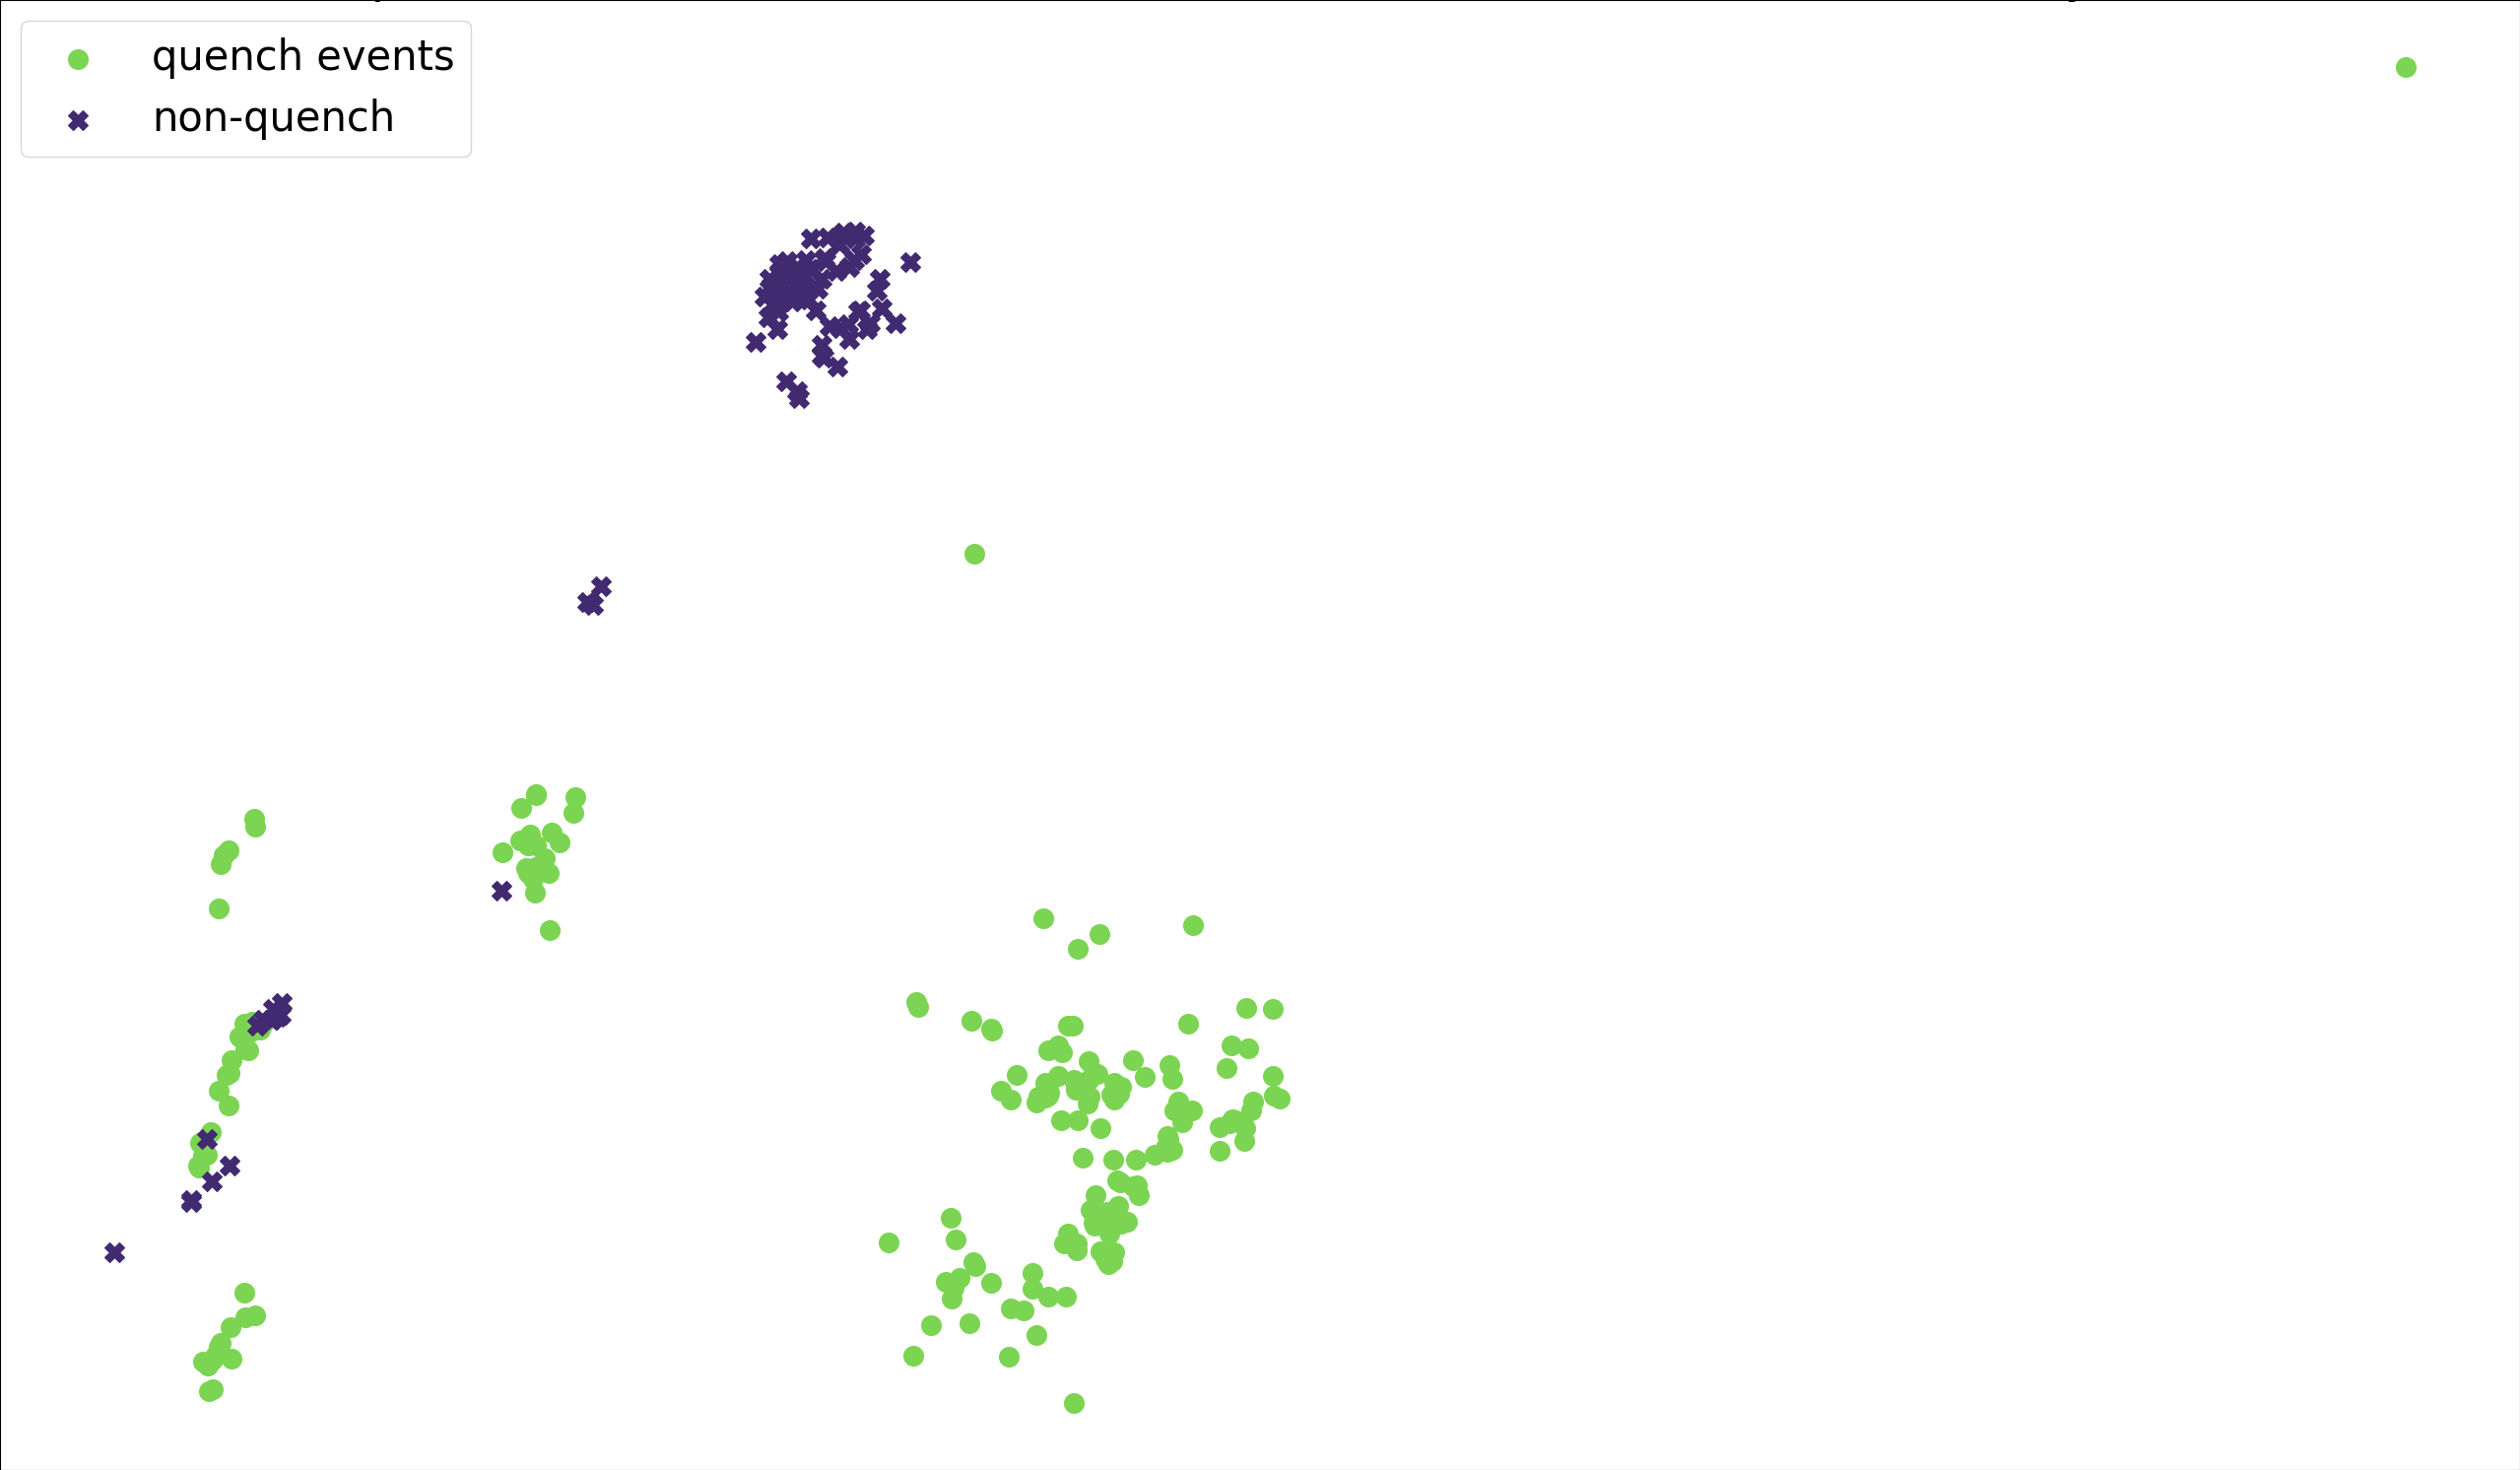
\includegraphics[width=\linewidth]{img/Cnmod_distribution.png}
	\caption{Data distribution for the \cnmod table after applying $\textsc{pca}$ dimensionality
		reduction} \label{fig:cnmod-dist}
\end{figure}
As we can see in \Cref{fig:cnmod-dist} the samples are characterized by a good enough distribution,
we could easily identify clusters with a high degree of purity, apart from the one in the leftmost
region of the image, which contains many points tagged as quench events and many points tagged as
non quenches.

\subsubsection{\phin table}
As we will see in further sections the \phin table did not perform exceptionally, but it consistently
outperformed the one based on \bn. I believe that, as we saw with \bn, the root of the bad performance
is standing in the fact that both tables have a high degree of homogeneity in the distribution of
the samples, this can be seen quite clearly in \Cref{fig:phi-dist}.

\begin{figure}[h!]
	\centering
	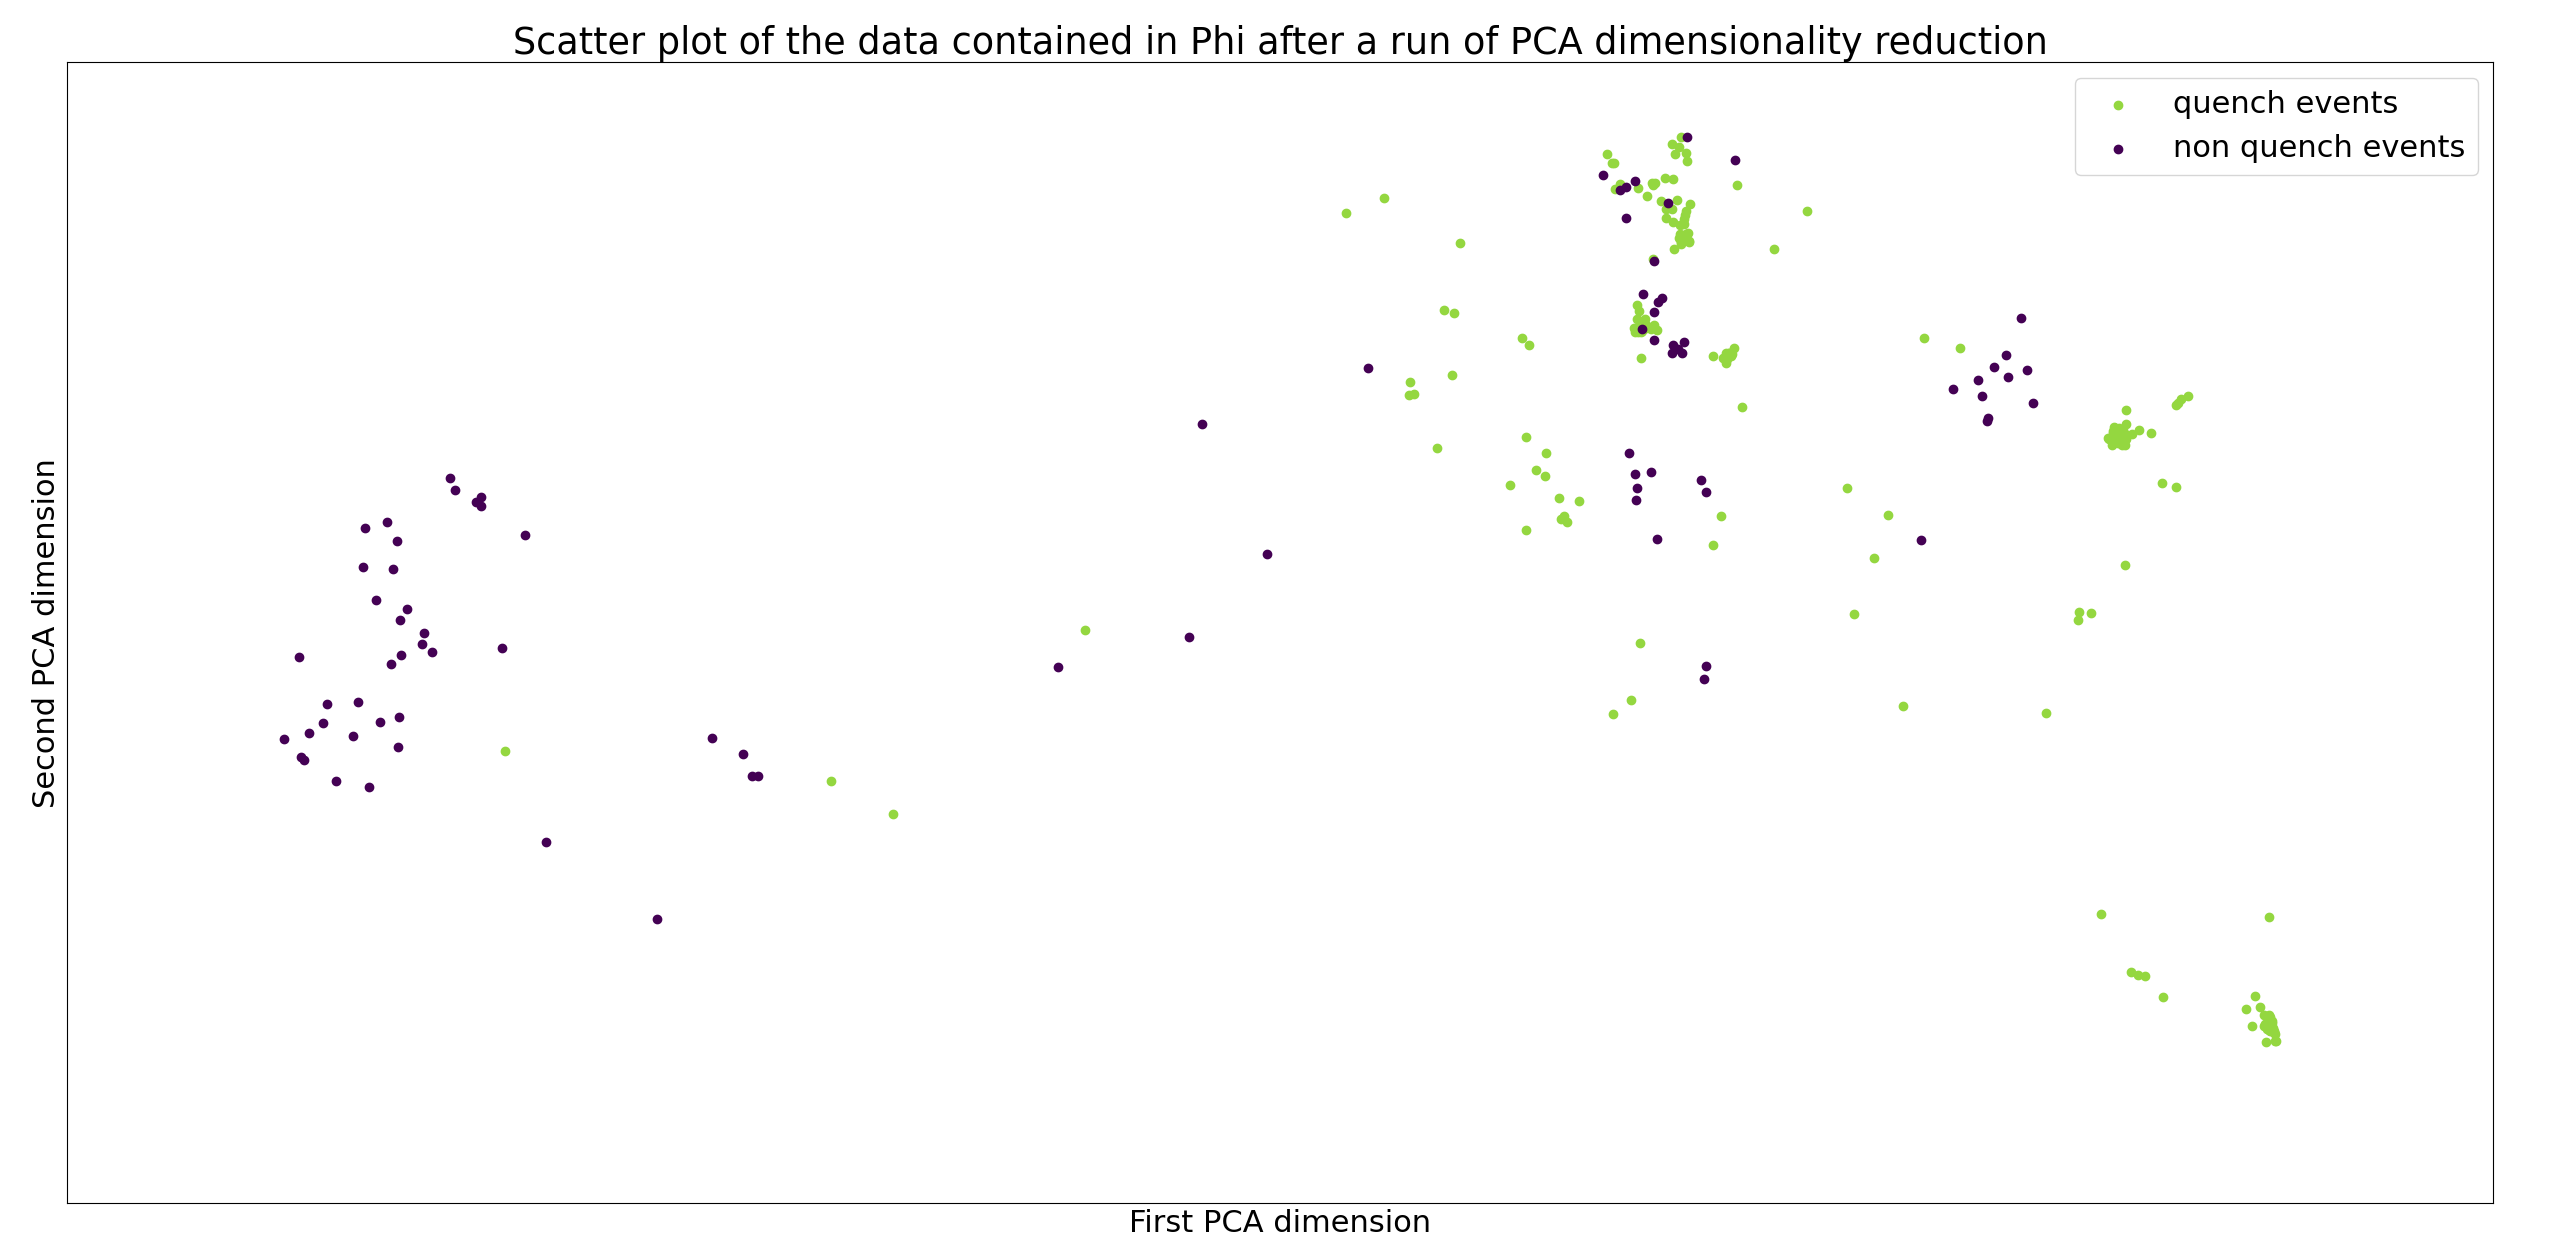
\includegraphics[width=\linewidth]{img/Phi_distribution.png}
	\caption{Data distribution for the \phin table after applying $\textsc{pca}$ dimensionality
		reduction} \label{fig:phi-dist}
\end{figure}

\medskip

As far as the correlation matrix is concerned we can see in \Cref{fig:phi-corr} that, contrarily to
the correlation matrix of other tables, the amount of harmonics that are strongly correlated with
each other is kept to a minimum. No real structure can be seen in this table as was the case of \an
and \bn.
\begin{figure}[h!]
	\centering
	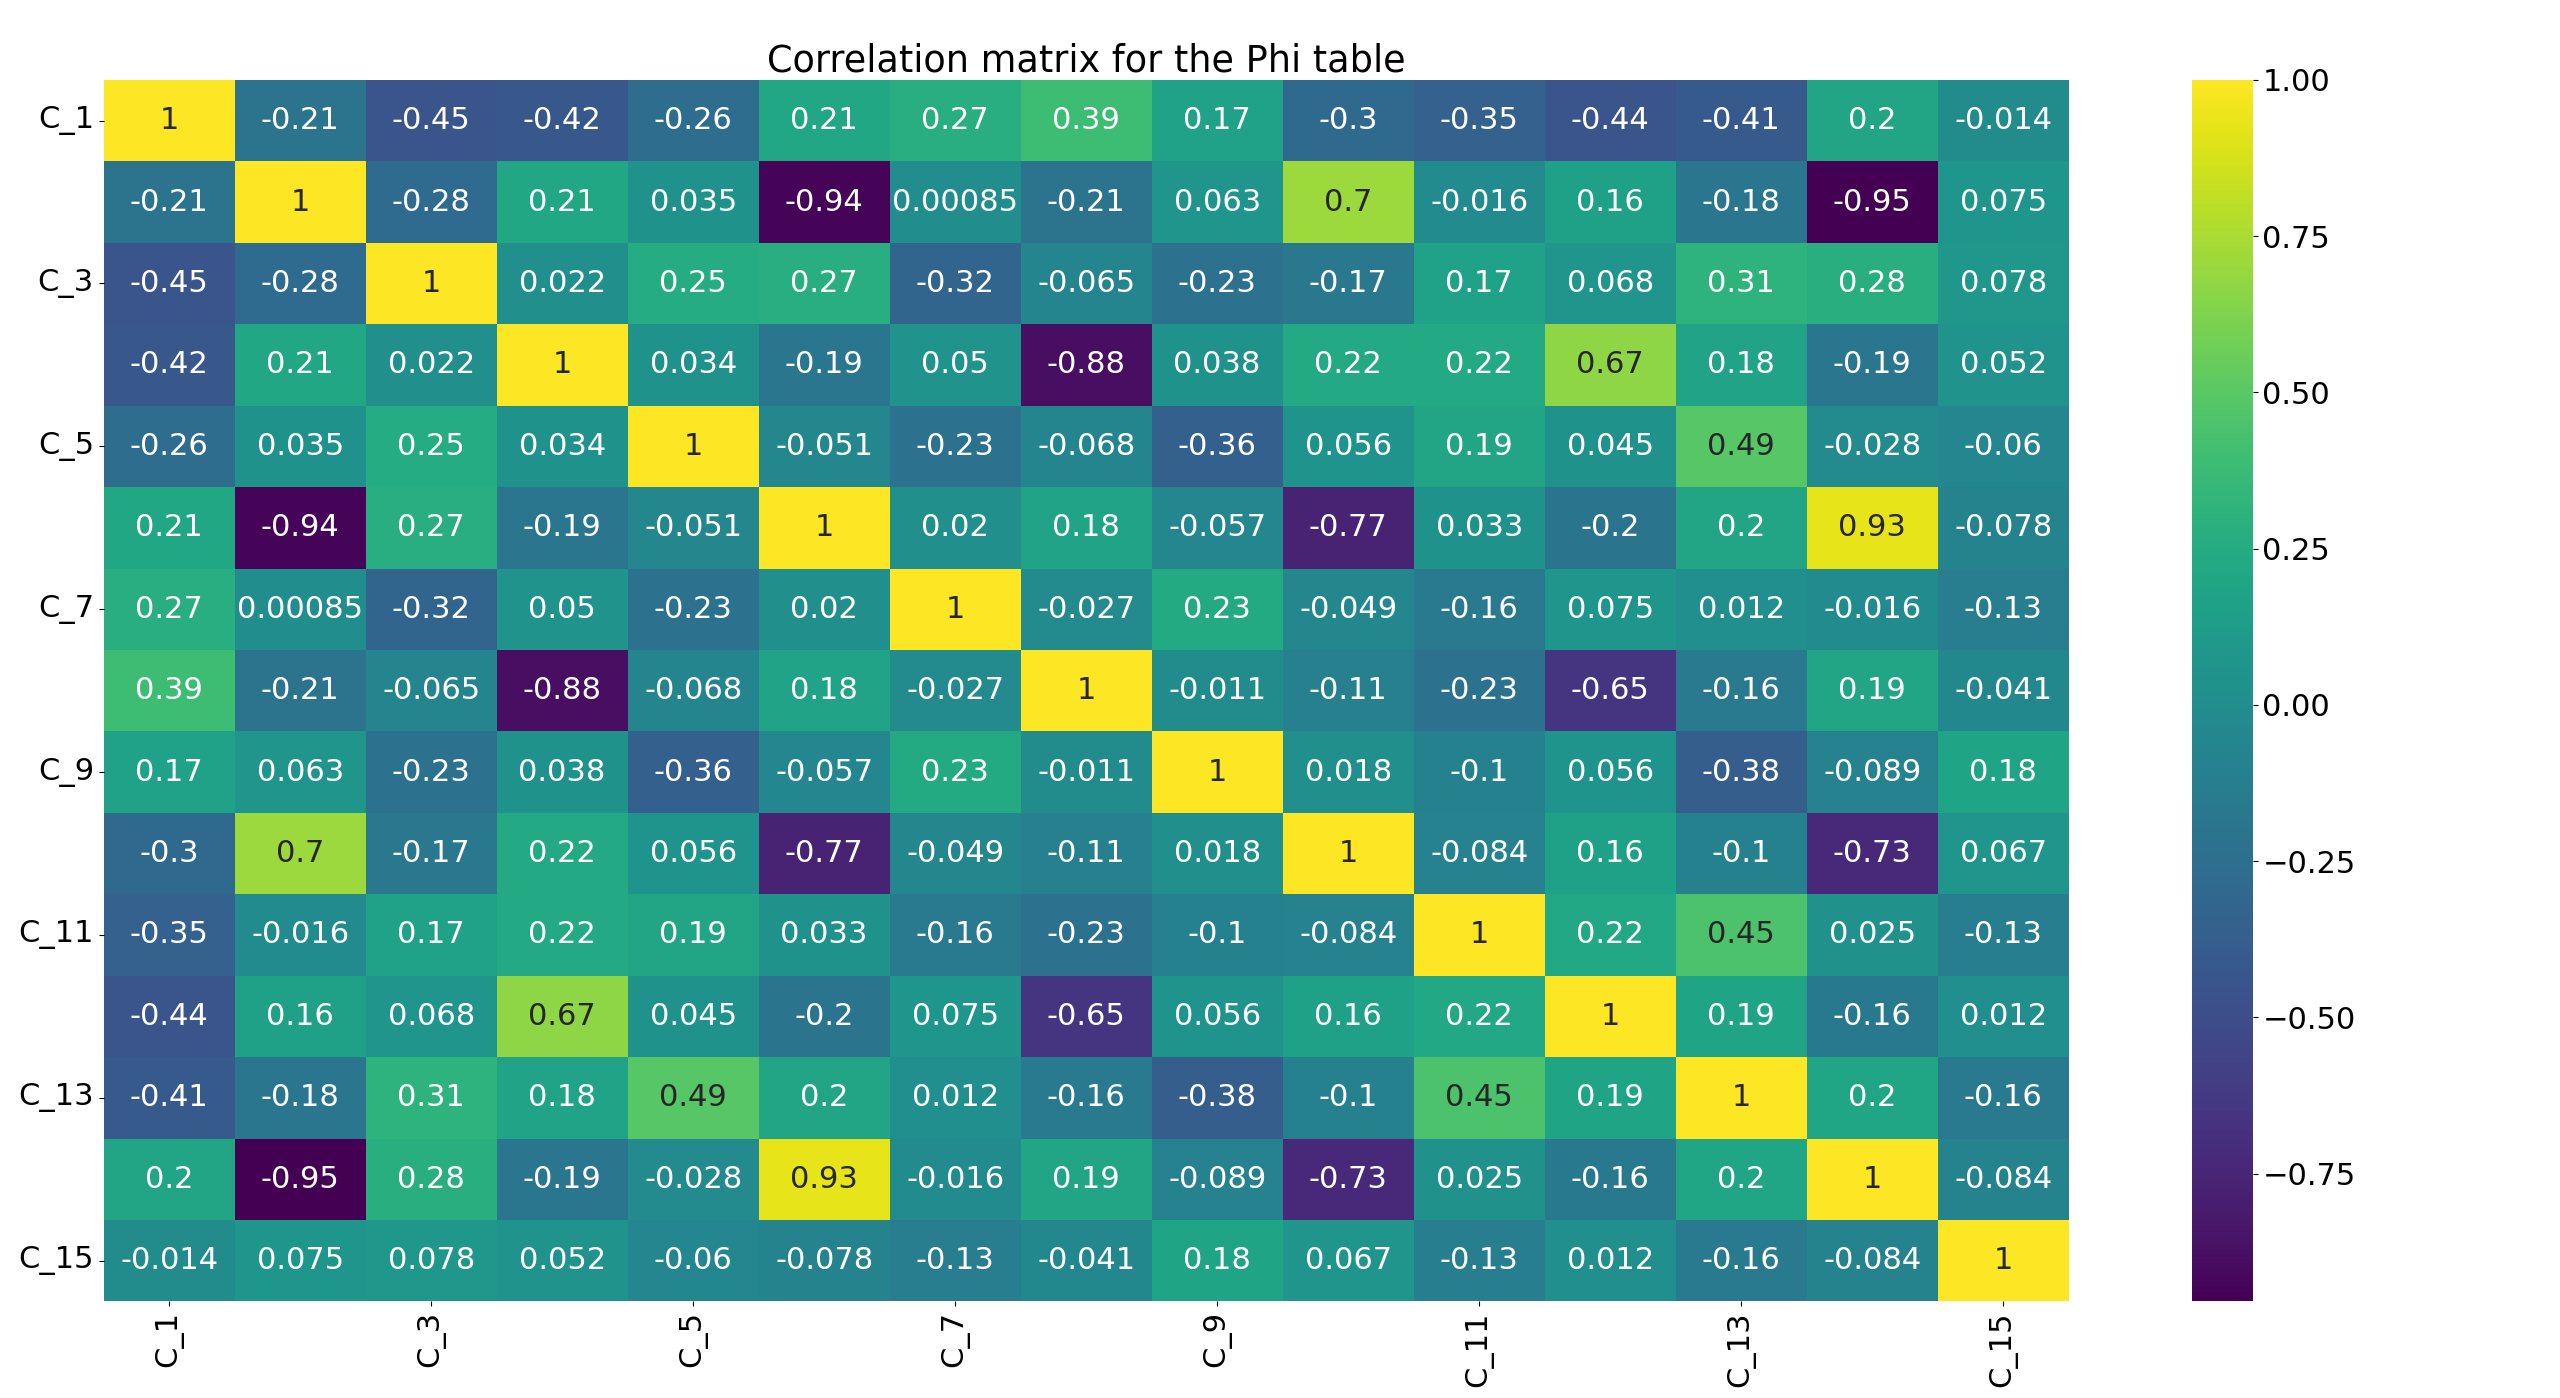
\includegraphics[width=\linewidth]{img/Phi_corr_matrix.png}
	\caption{The cross-correlation of the \phin harmonics} \label{fig:phi-corr}
\end{figure}
This structure leaves us with much more freedom as to which harmonics to pick to build datasets
(compared with \an, \bn and \cnmod), the only things that really stand to the eye are that: harmonic
number $2$ is strongly correlated with its odd multiples, harmonic number $4$ is strongly correlated
with its multiples.

Lastly, we can analyze the correlation between the harmonics and the label. As we can see in \Cref{fig:phi-lcorr} most of the harmonics have a good correlation with the expected solution, especially harmonic number $2$ and its odd multiples, and harmonics number $1$ and $12$.
\begin{figure}[h!]
	\centering
	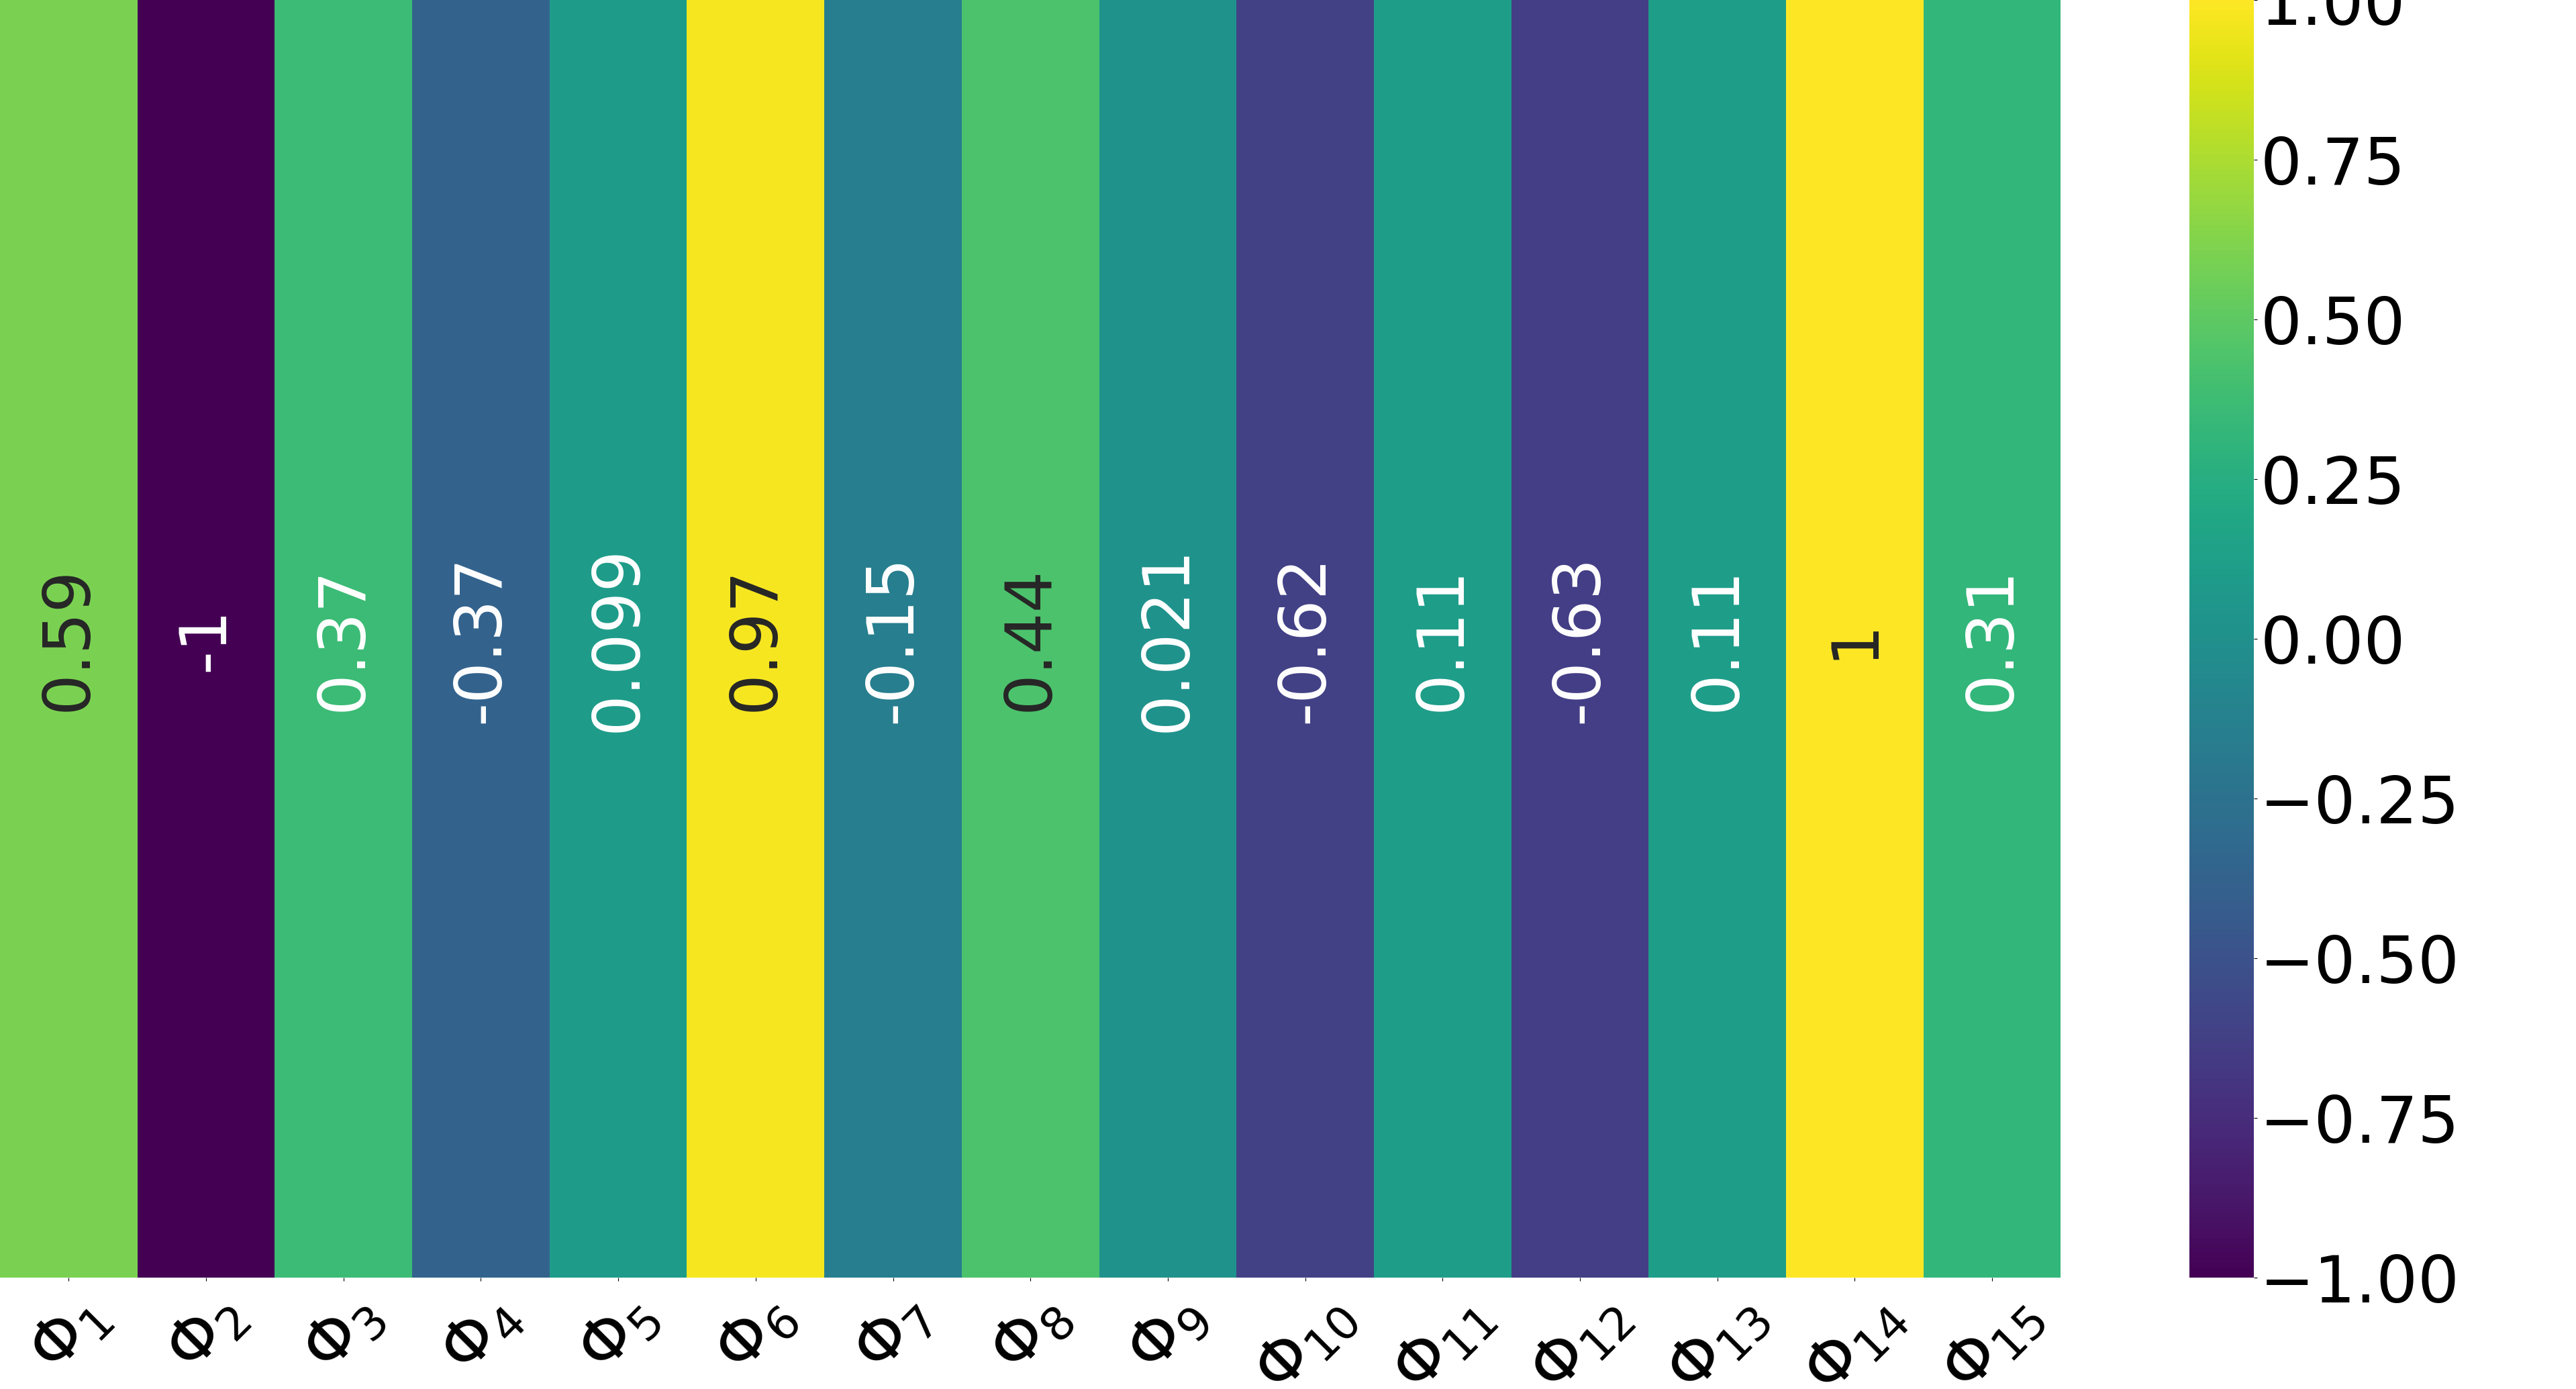
\includegraphics[width=\linewidth]{img/Phi_label_corr.png}
	\caption{Label correlation for the \phin table} \label{fig:phi-lcorr}
\end{figure}
This closes the brief exposition about the preprocessing steps for the various labels, now we will
tackle the model selection procedure indicating which were the best models overall and which model
we chose to solve $\qrp$.

\section{Results}
Every model shown in this section has been tested using the pipeline that I talked about in
\Cref{chp:problem}, due to some changes done around the time of writing, hyperparameter tuning has
been done with $\ncv$ using both the normal randomized KFold as well as StratifiedKFold. While the
performance difference is not as important as one might imagine, the final results were different
enough to push me to move the pipeline to the use of StraifiedKFold. In the following I will only
provide results for the models obtained using stratified sampling for fold construction and I will
provide a comparison of the performance metrics only when the difference is deemed appreciable.

\subsection{Decision trees}
As we already alluded to in previous sections we wanted to find a highly explainable model with good
performance that could be used to solve $\qrp$.

We tried many different approaches where various tables were involved and different harmonics were
being used, but the best table always remained \an, which performance are shown in
\Cref{fig:dt-an-2-12-15-perf}. As we can see, even if we use the simple decision tree model, we are
capable of explaining whether a sample is 'quench' or 'non quench' by using a very limited amount of
harmonics (only three are necessary).
\begin{figure}[h!]
	\centering
	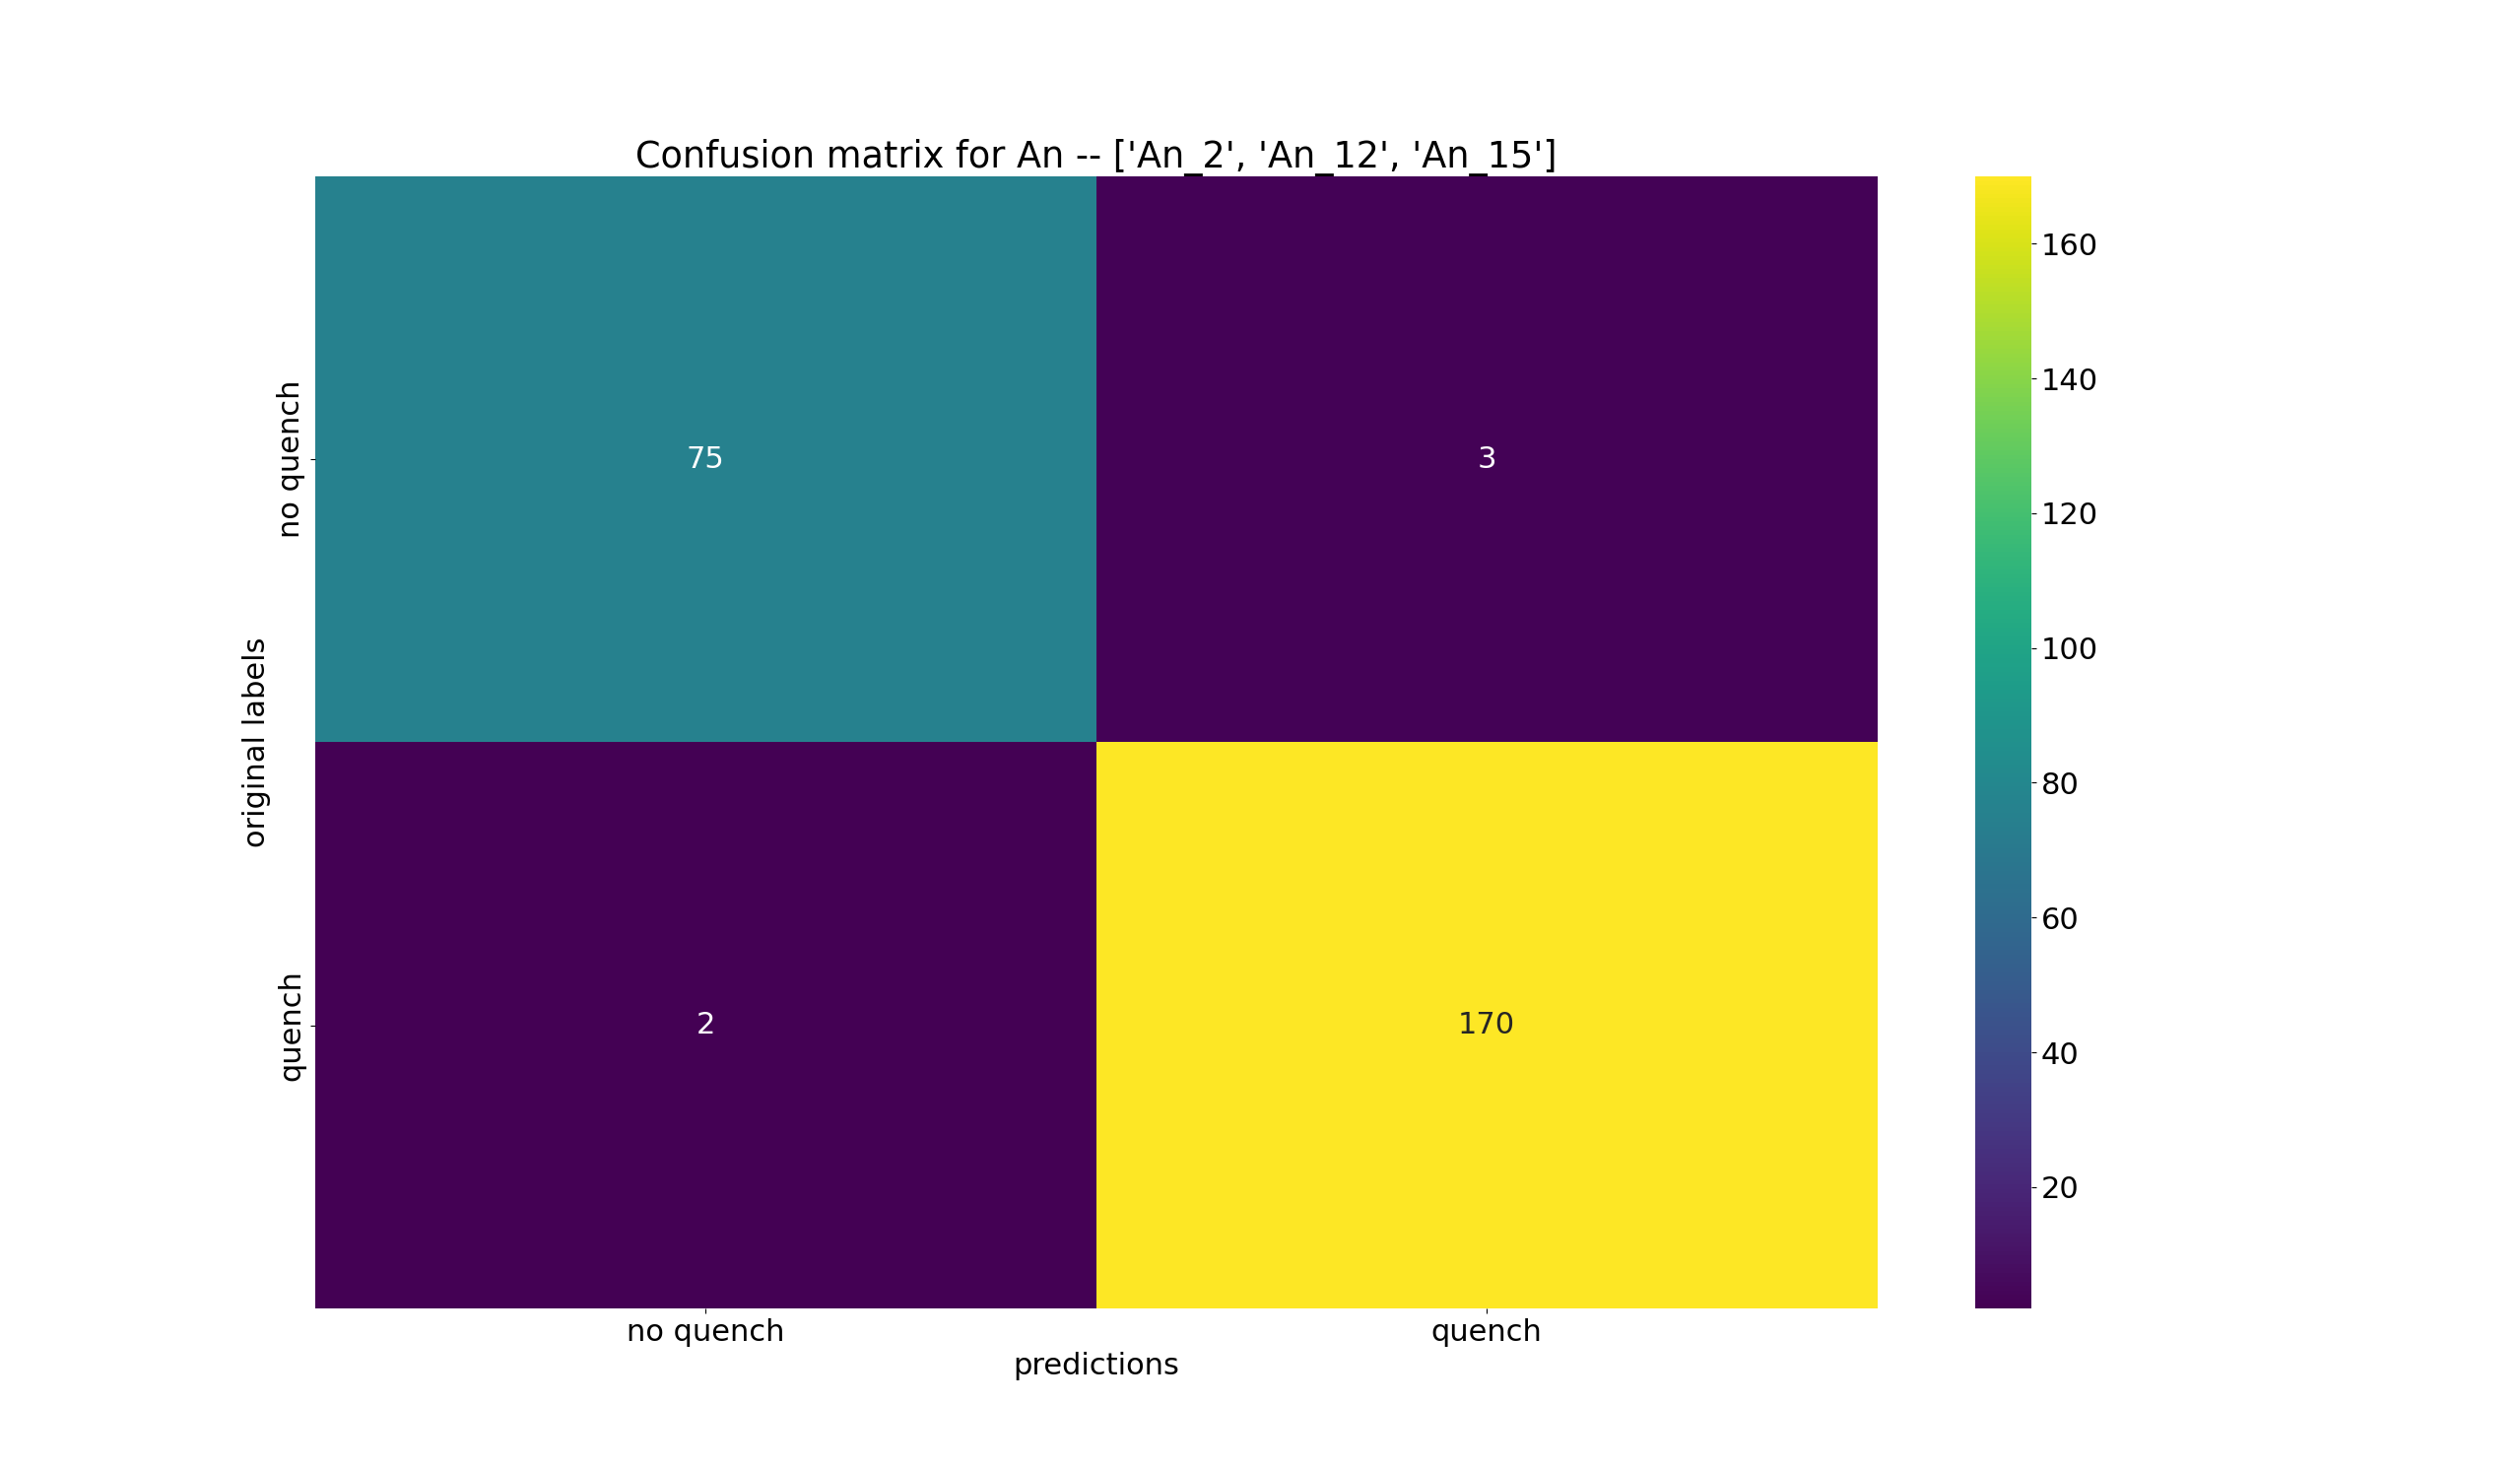
\includegraphics[width=\linewidth]{img/An_2_12_15_cm_dt.png}
	\caption{The performance for the \an model built on harmonics $2, 12, 15$} \label{fig:dt-an-2-12-15-perf}
\end{figure}
If we look at \Cref{fig:dt-an-2-12-15-pt}, we can see that the structure of the tree is also
extremely simple, contained in depth, using mostly harmonic number $2$ to perform the splits and
having only one node where the impurity is not zero.
\begin{figure}[h!]
	\centering
	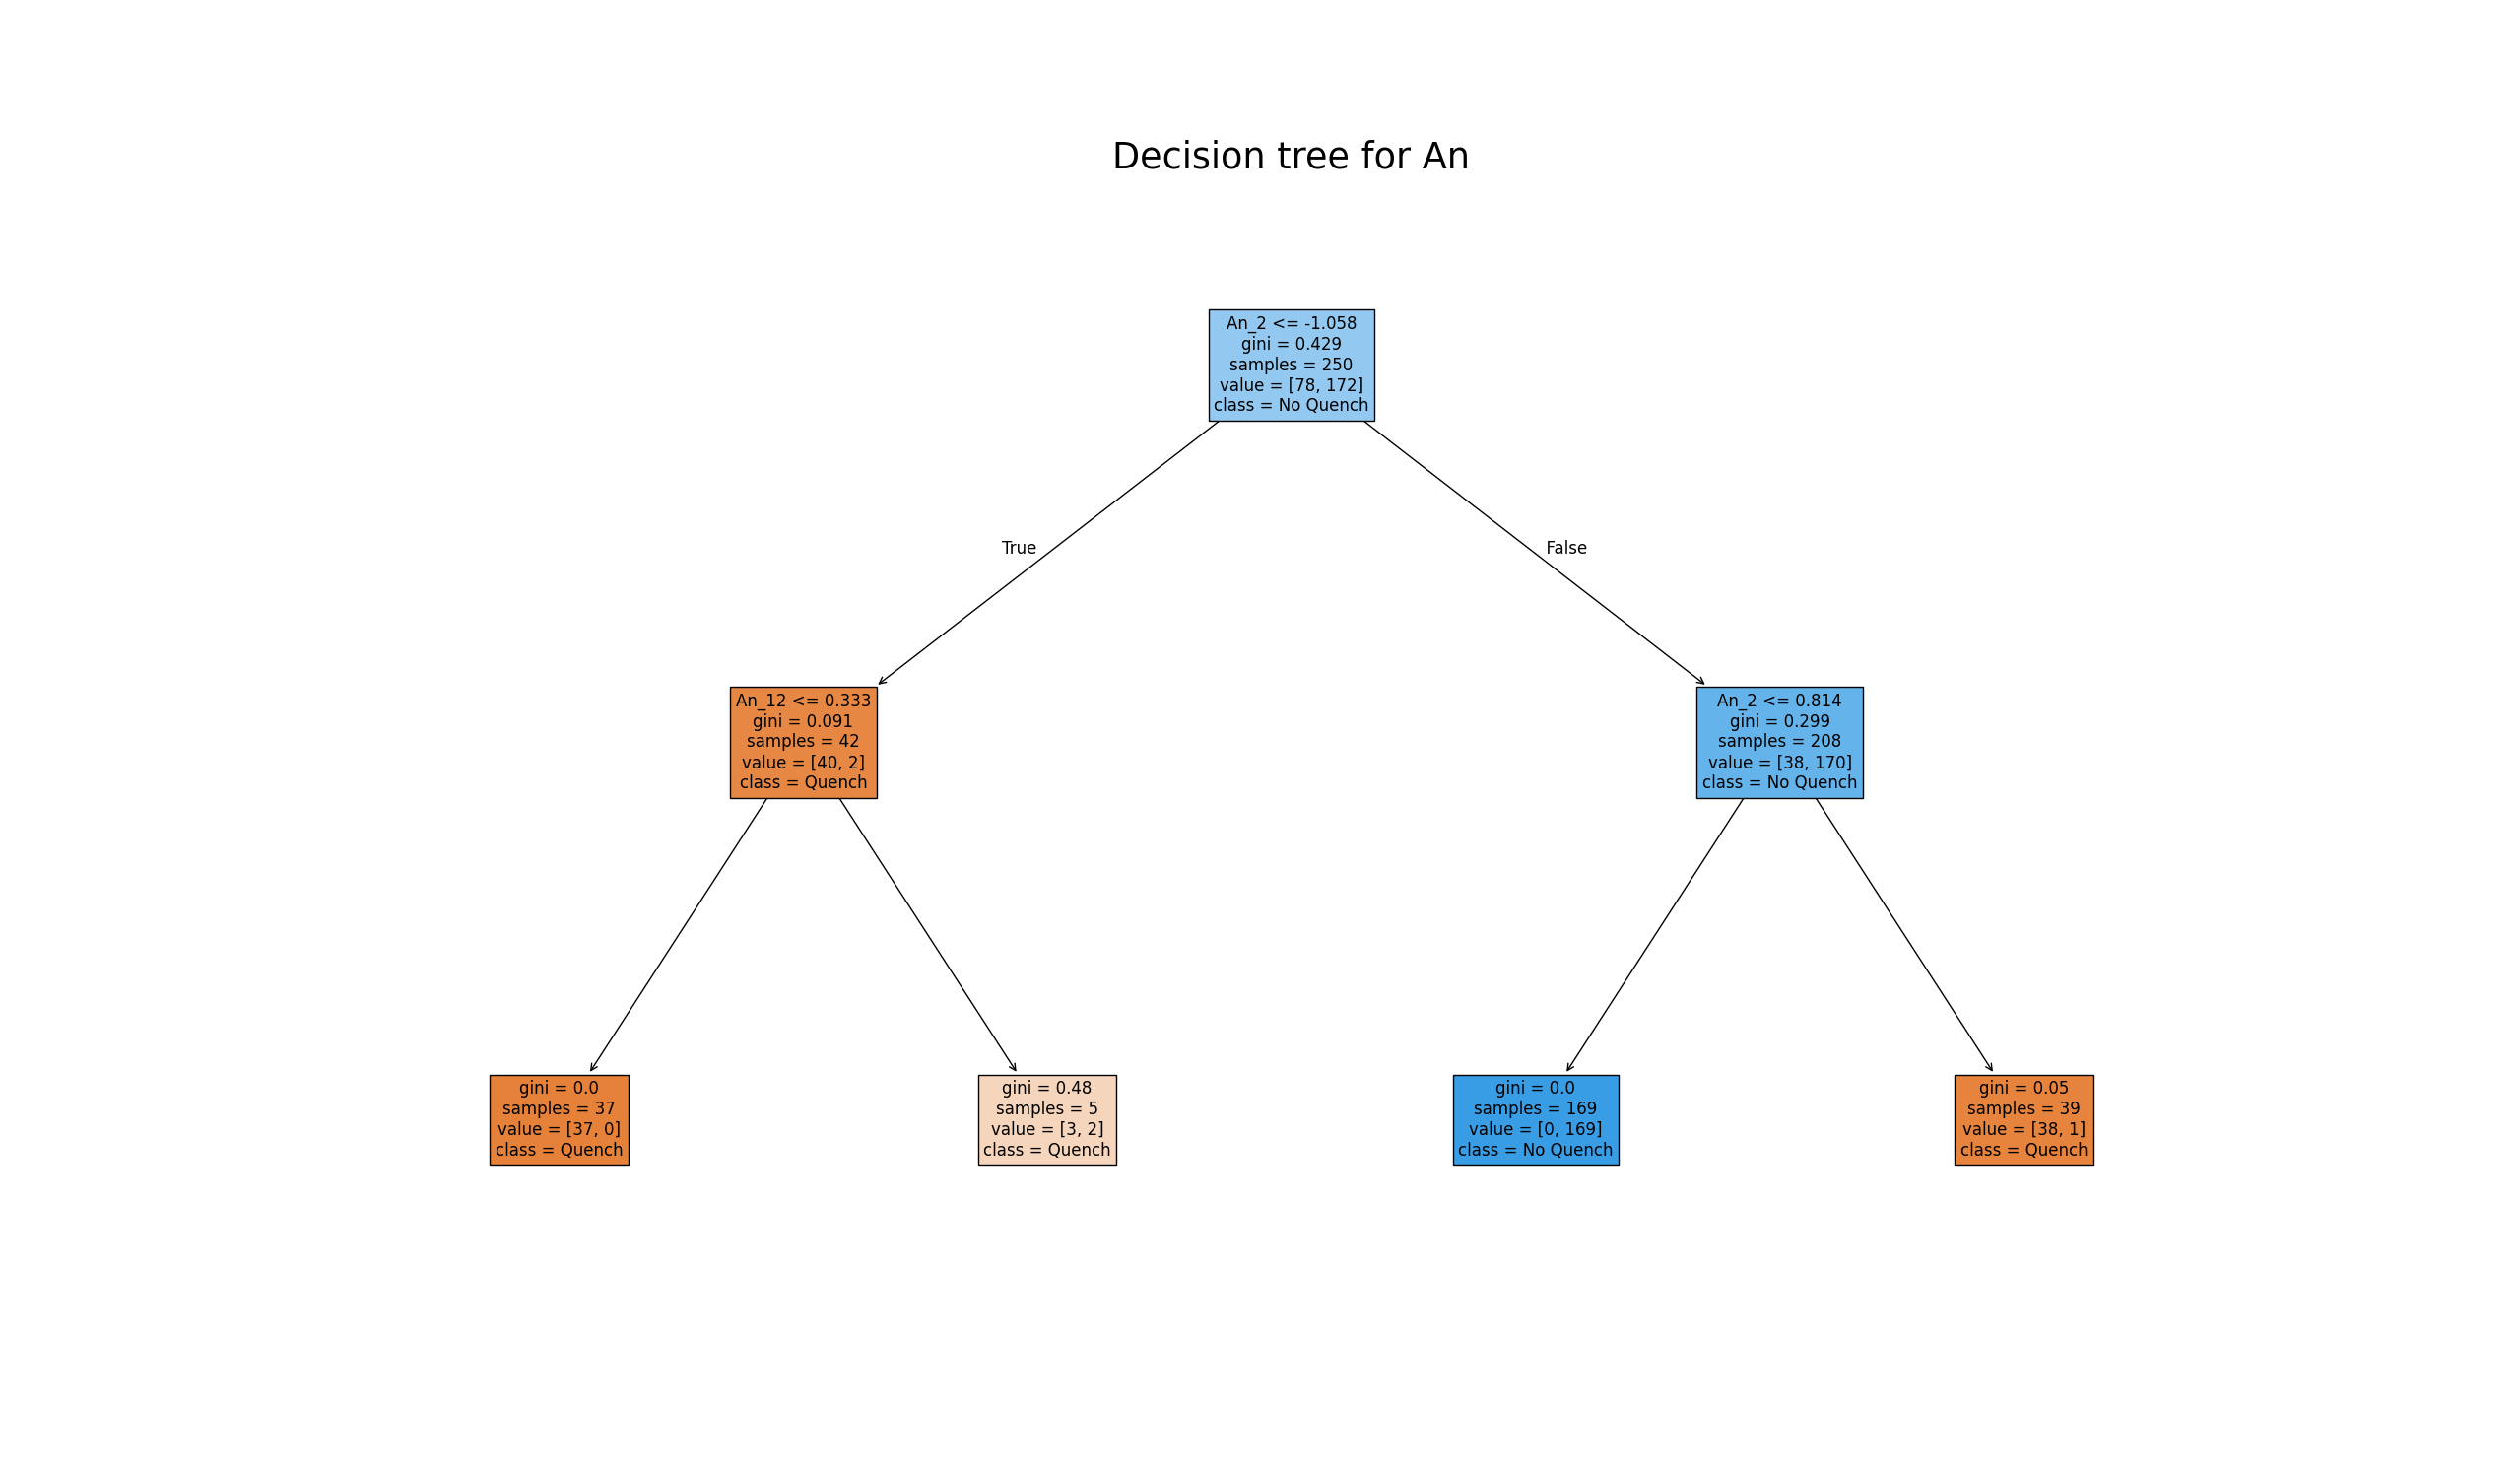
\includegraphics[width=\linewidth]{img/An_2_12_15_pt_dt.png}
	\caption{The structure of the tree built on harmonics $2, 12, 15$} \label{fig:dt-an-2-12-15-pt}
\end{figure}
Many were the models tested in this phase but all of them fell short of the performance of the model
shown in \Cref{fig:dt-an-2-12-15-pt}, that is enough of a reason why, we will not be covering them
in depth. All we will do is plot the performance of the best decision tree built on every table to
compare them against each other.
\begin{figure}[h!]
	\centering
	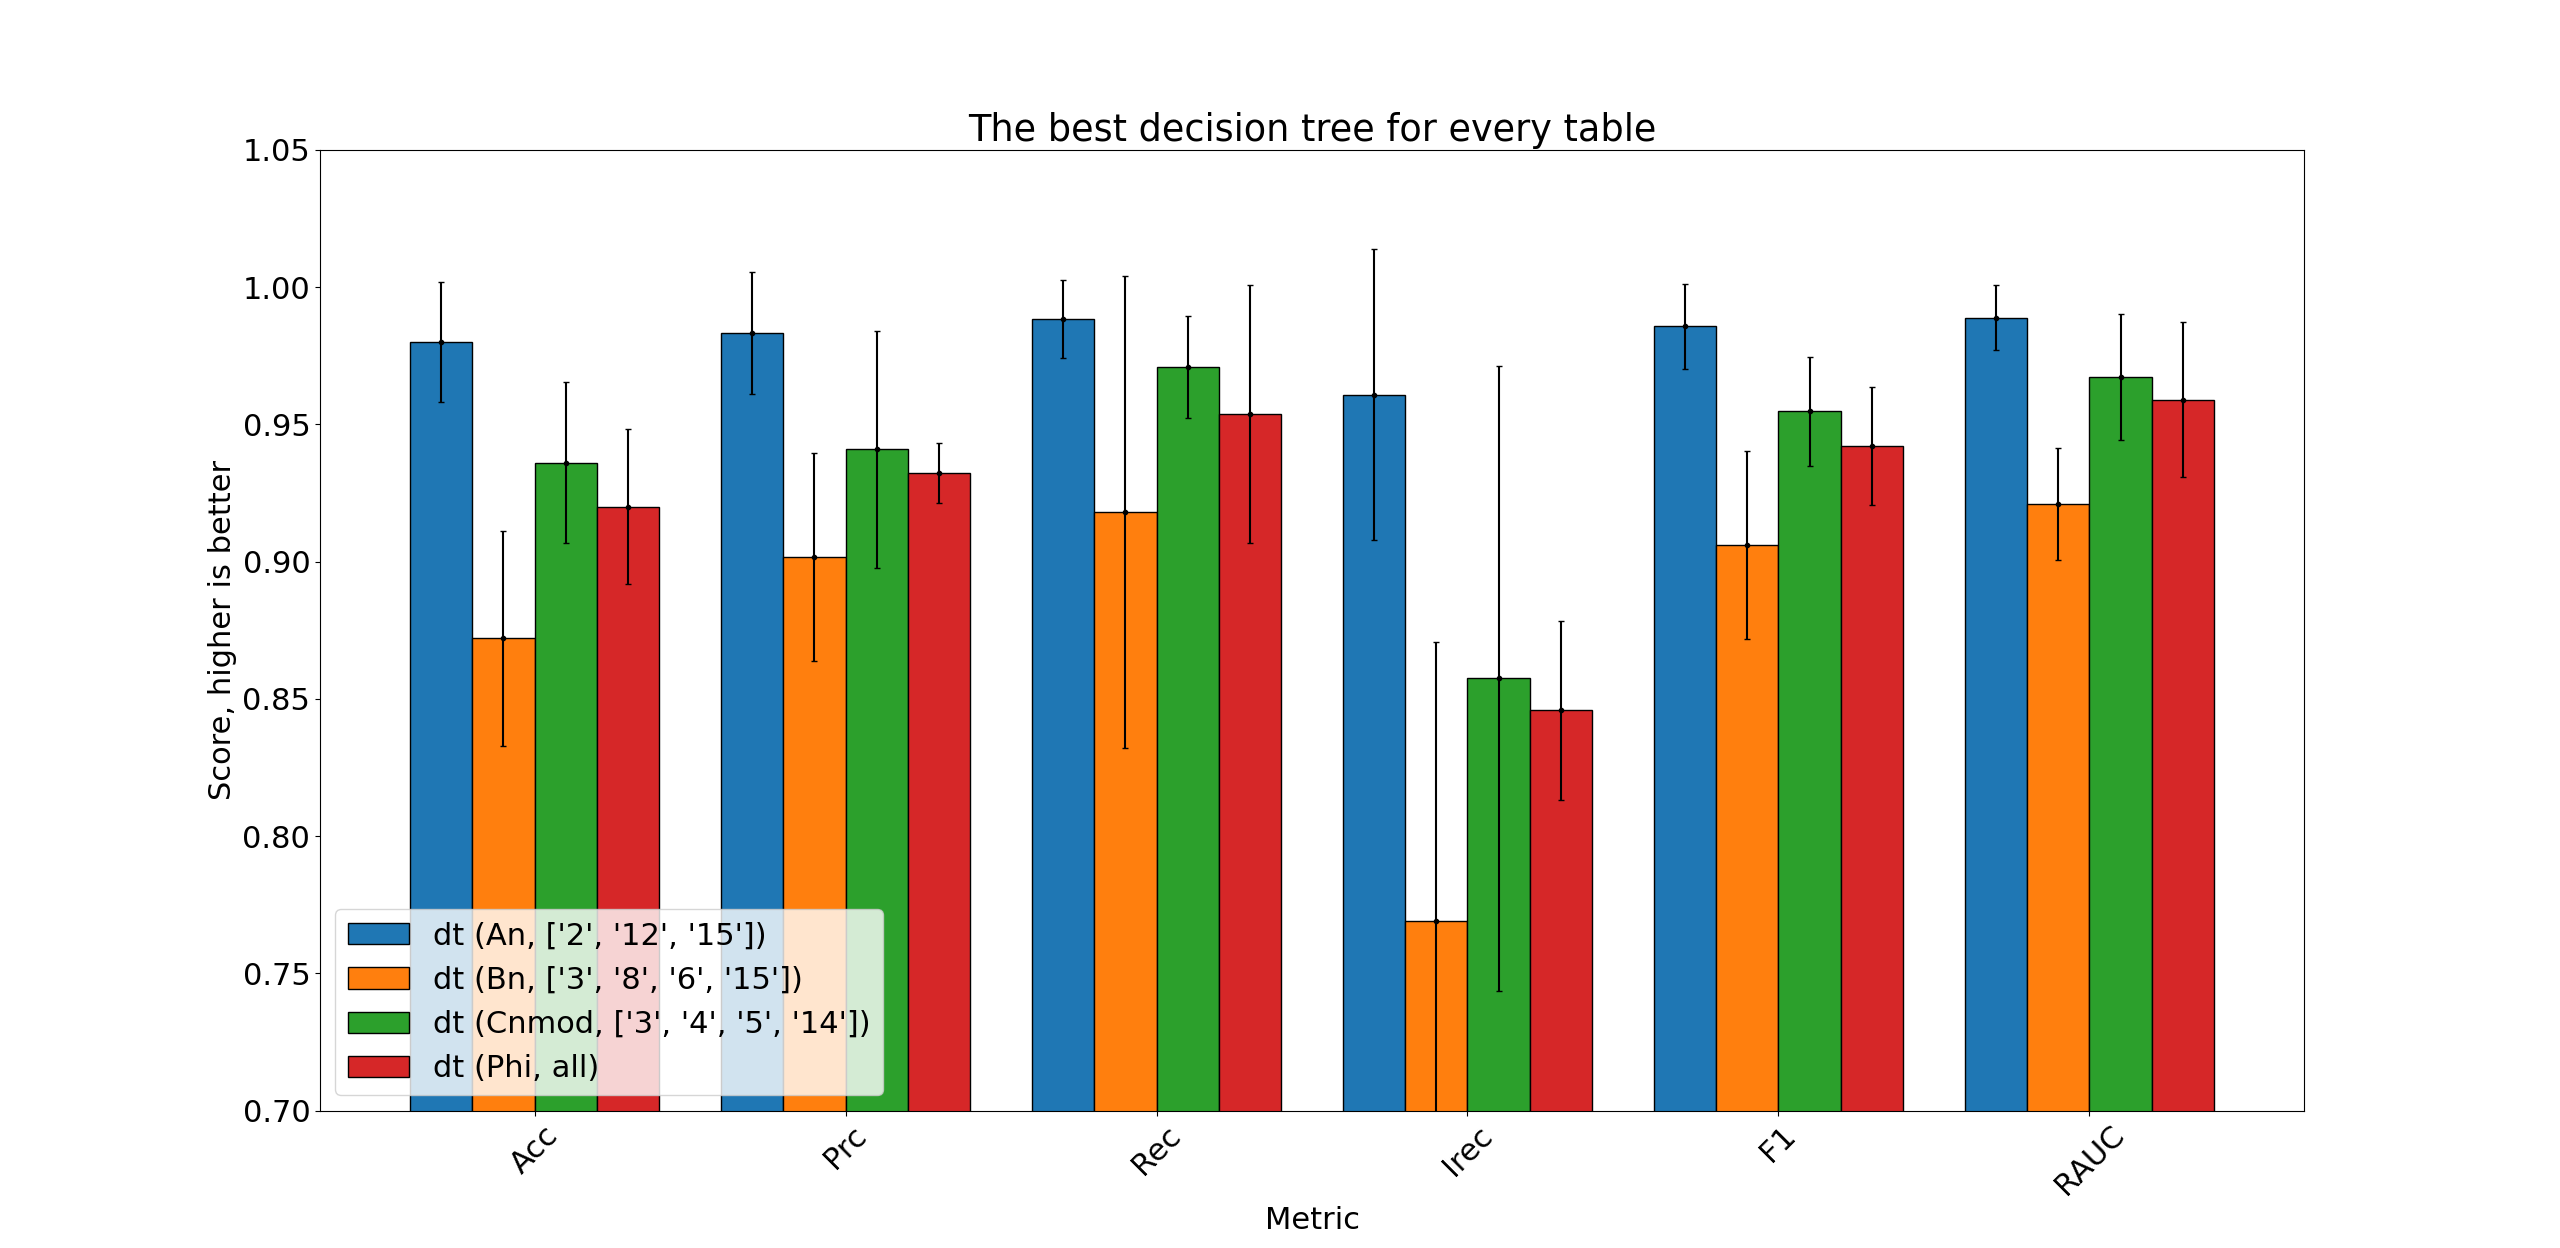
\includegraphics[width=\linewidth]{img/best_dts.png}
	\caption{Performance comparison of all the best decision trees} \label{fig:best-dts}
\end{figure}

As we can see in \Cref{fig:best-dts}, the performance for the best models built on tables \bn, \cnmod
and \phin, are worse than the ones obtained by using \an, and the margin is quite important.
\subsection{SVM}
Before moving onward to the other models let's consider the $\svm$, as we said in \Cref{sec:svm}, it
is a very high performance model, capable of finding the solution with a very high accuracy. All of
this is done my transposing the samples to a higher dimensional space where a dividing hyperplane
can be found. Since this mapping is unknown and we are using an approximation for it, the $\svm$
model has a very low degree of explainability.

The reason why we are introducing the $\svm$ model first is because we got very high performance out
of decision trees already, therefore we asked ourselves what was the best performance we could be
pushing for. If we compare the best $\svm$ with the best decision tree, like we did in
\Cref{fig:svm-vs-dt}, it's clear that there is still quite a bit of room for improvement, especially in the Inverse recall metric, which is the one where most models are at fault.
\begin{figure}[h!]
	\centering
	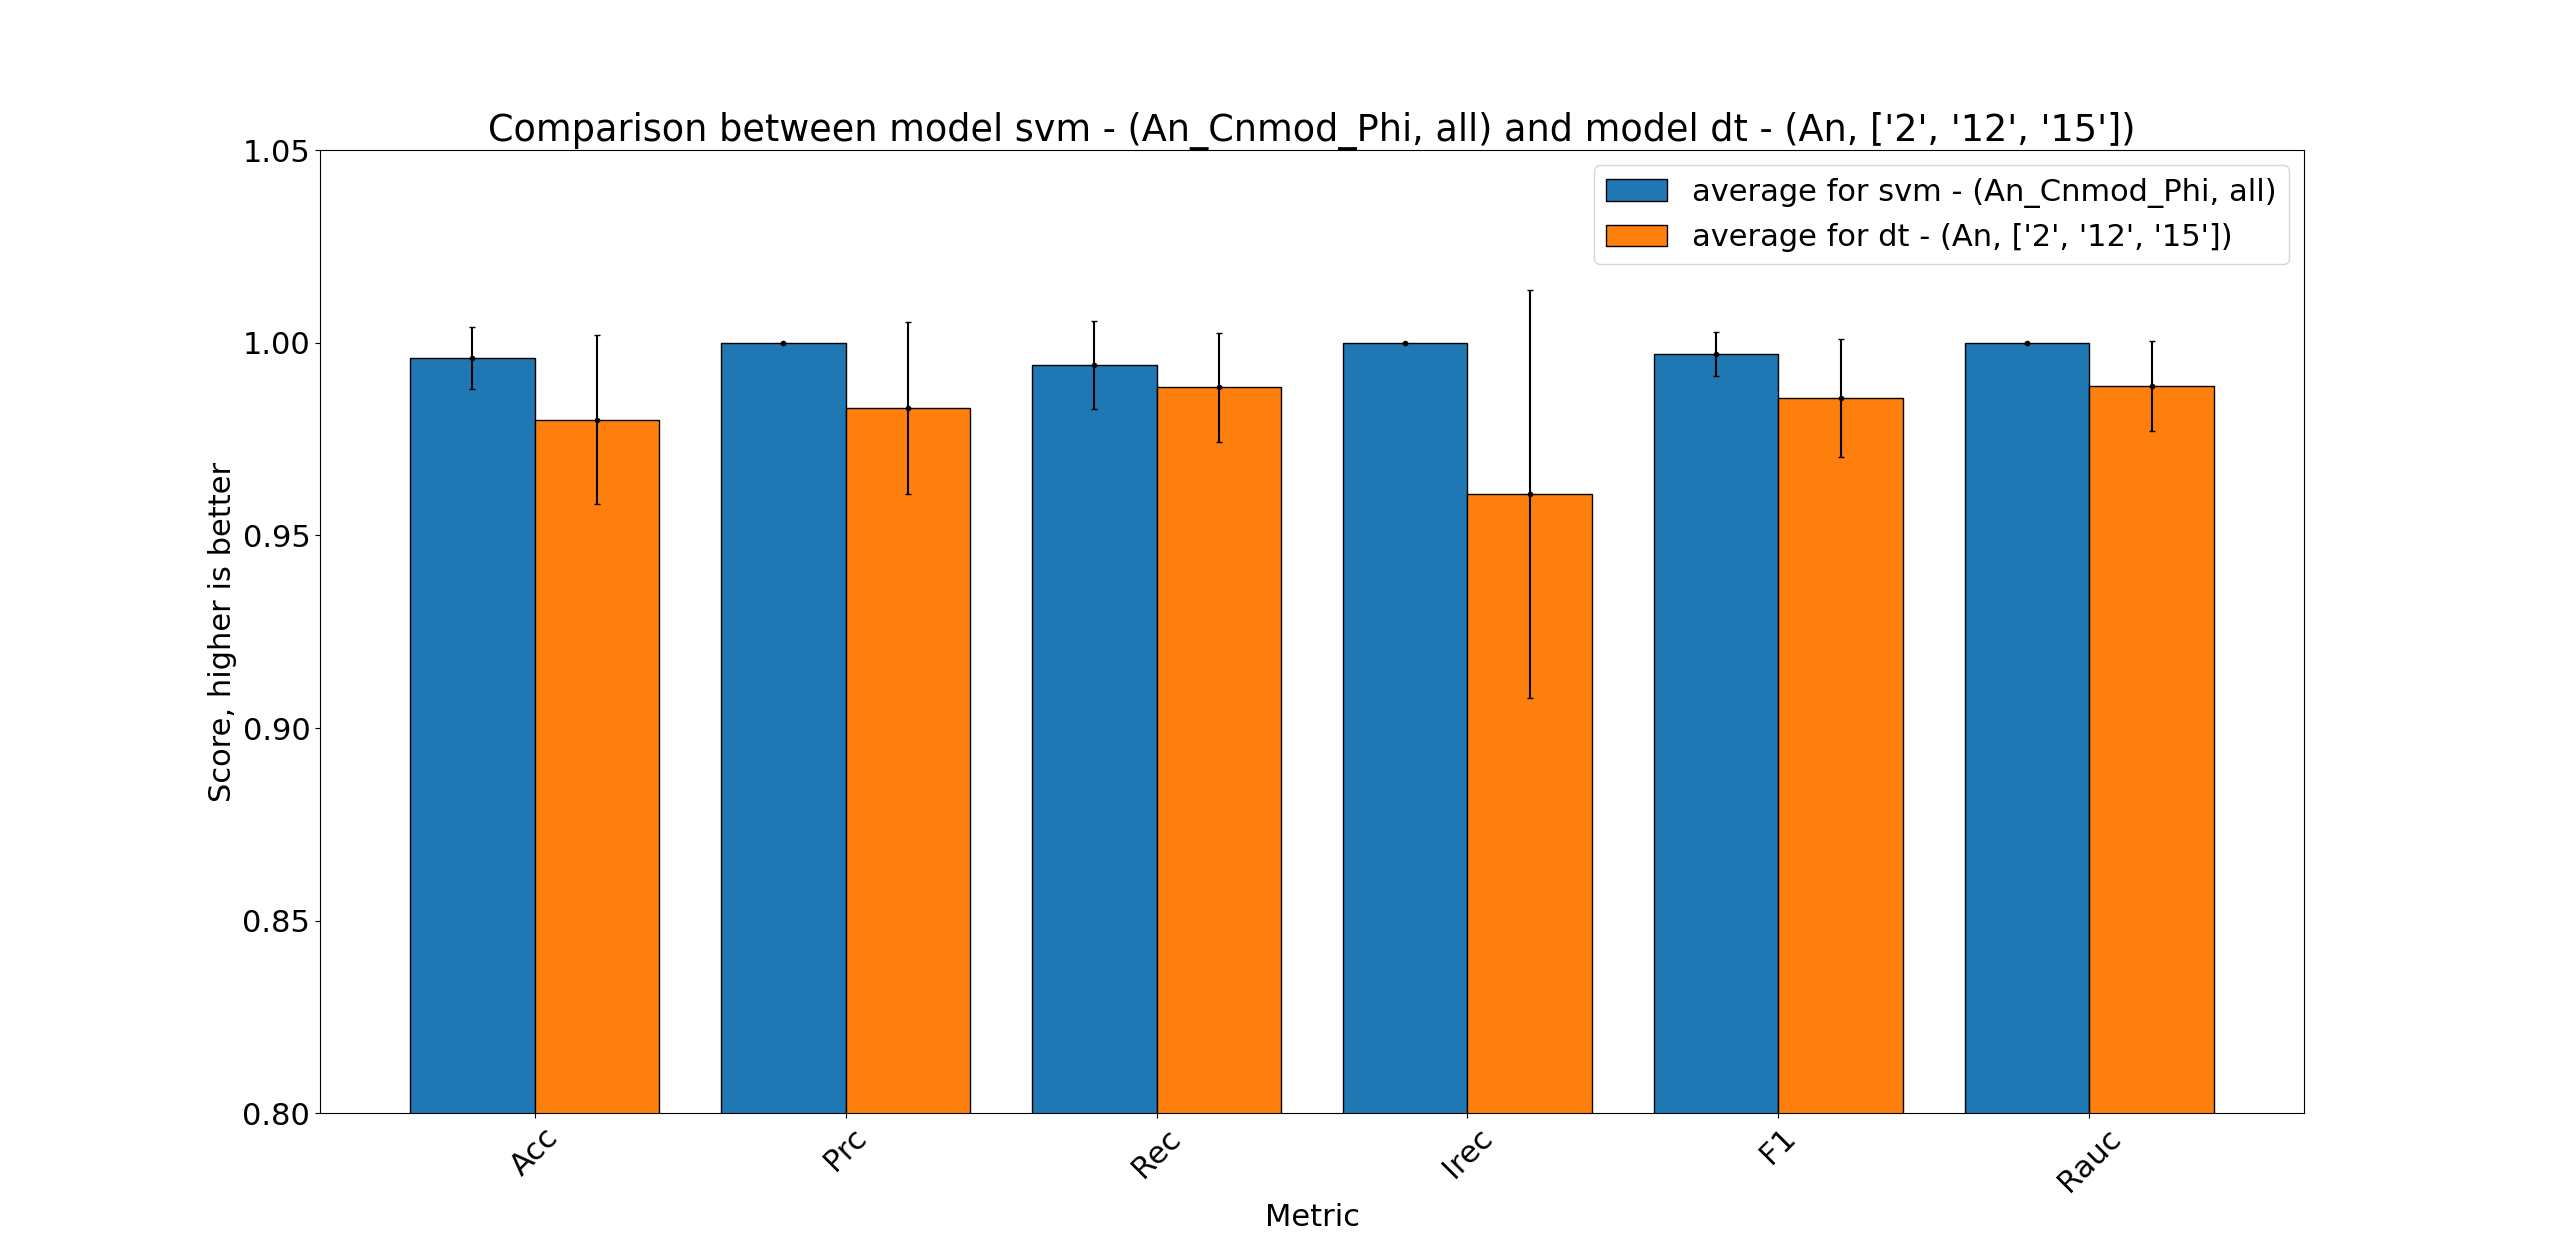
\includegraphics[width=\linewidth]{img/svm_vs_dt.png}
	\caption{Performance comparison of $\svm$ and decision tree} \label{fig:svm-vs-dt}
\end{figure}
The model that are shown in this plot are:
\begin{itemize}
	\item The decision tree we just introduced (\Cref{fig:dt-an-2-12-15-pt}),
	\item The $\svm$ is built on top of a mix of tables (\an, \cnmod and \phin), using the full
	      harmonic content, a polynomial kernel of degree $3$, with a regularization parameter
	      of $0.1$ and a kernel coefficient $\gamma = 0.1$ and a $c_0 = 0.1$. Both of these
	      hyperparameters were not introduced in \Cref{sec:svm} because they are
	      implementation specific, as a matter of fact, the polynomial kernel has the
	      following structure $\kappa(x, y) = (\gamma\trans{\vec{x}}y + c_0)^d$.
\end{itemize}

In the following we will be showing two different techniques, still based on trees, which yielded
very high performance and we will later close the chapter with an analysis of the model that we
chose to solve the problem performed the best overall.

\subsection{Random Forests}

\subsection{Tree Aggregators}

\subsubsection{Performance on the triplets}
